% !TeX root = rapportCS.tex
% Cœur scientifique exhaustif, rédigé en français et intégré au corps
% principal du rapport. Il présente la chaîne de calcul dans un ordre
% pédagogique : données microscopiques, transformations analytiques, fermeture
% auto-cohérente, algorithmes, paramètres et contrôles de reconstruction.

% =============================================================================
\section{Du Hamiltonien effectif discret au modèle continu}
\label{ann:hamiltonien_continu}
% =============================================================================

Ce chapitre constitue le début du cahier de calcul. Il est volontairement plus
détaillé qu'une présentation destinée à un article : le lecteur doit pouvoir
repartir des paramètres publiés
\hyperref[sec:core_parameter_sets]{\textcolor{blue}{(Annexe~A)}}, vérifier les
facteurs de volume et reconstruire le noyau envoyé au solveur. Pour chaque transformation, je donne l'expression
discrète, l'opération effectuée et l'objet implémenté.

\subsection{Préambule : origine du modèle et conventions}
\label{sec:origin_dft}

\noindent\textbf{Origine DFT du modèle.}
Le Hamiltonien effectif microscopique est construit à partir de calculs
\emph{ab initio} menés dans le cadre de la théorie de la fonctionnelle de la
densité (DFT). Son principe est de décrire l'état fondamental électronique par
la densité $n(\mathbf r)$ plutôt que par la fonction d'onde de tous les
électrons. Dans la formulation de Kohn--Sham, la minimisation de l'énergie,
considérée comme une fonctionnelle de $n(\mathbf r)$, fournit la densité et
l'énergie totale pour une configuration donnée des ions.

En répétant ce calcul pour un ensemble de structures légèrement déformées, on
obtient les variations d'énergie et les forces associées aux déplacements
atomiques. Ces données permettent d'ajuster les constantes de force, les
couplages anharmoniques et les couplages à la déformation ; les charges
effectives et la réponse diélectrique électronique fixent la partie dipolaire.
Le Hamiltonien utilisé ici n'est donc pas la DFT elle-même, mais une
paramétrisation de basse énergie obtenue par projection des résultats DFT sur
un petit nombre de degrés de liberté pertinents~\cite{Zhong1994}.

\subsubsection{Transition paraélectrique--ferroélectrique}
\label{sec:core_effective_coefficients}

La polarisation est le paramètre d'ordre naturel de la transition
paraélectrique--ferroélectrique. Pour en visualiser le mécanisme, considérons
une seule de ses composantes, $P(\mathbf x)$, évaluée en un point \(\mathbf x\)
de l'espace, et le potentiel local scalaire le plus simple compatible avec
l'inversion $P\mapsto-P$,
\begin{equation}
V(P)=\frac{\alpha}{2}P^2+\frac{\beta}{4}P^4,
\qquad \beta>0.
\label{eq:core_local_landau_potential}
\end{equation}
La figure~\ref{fig:core_landau_double_well} représente cette énergie locale,
et non un profil spatial complet de polarisation. Lorsque $\alpha>0$, son
minimum unique est $P=0$ : la phase est paraélectrique et respecte la symétrie
d'inversion. Lorsque $\alpha<0$, le minimum central devient instable et deux
minima dégénérés apparaissent en $P=\pm\sqrt{-\alpha/\beta}$. Dans la limite
thermodynamique, le choix d'un de ces deux états par un domaine ferroélectrique
brise spontanément la symétrie $P\mapsto-P$.

\begin{figure}[htbp]
\centering
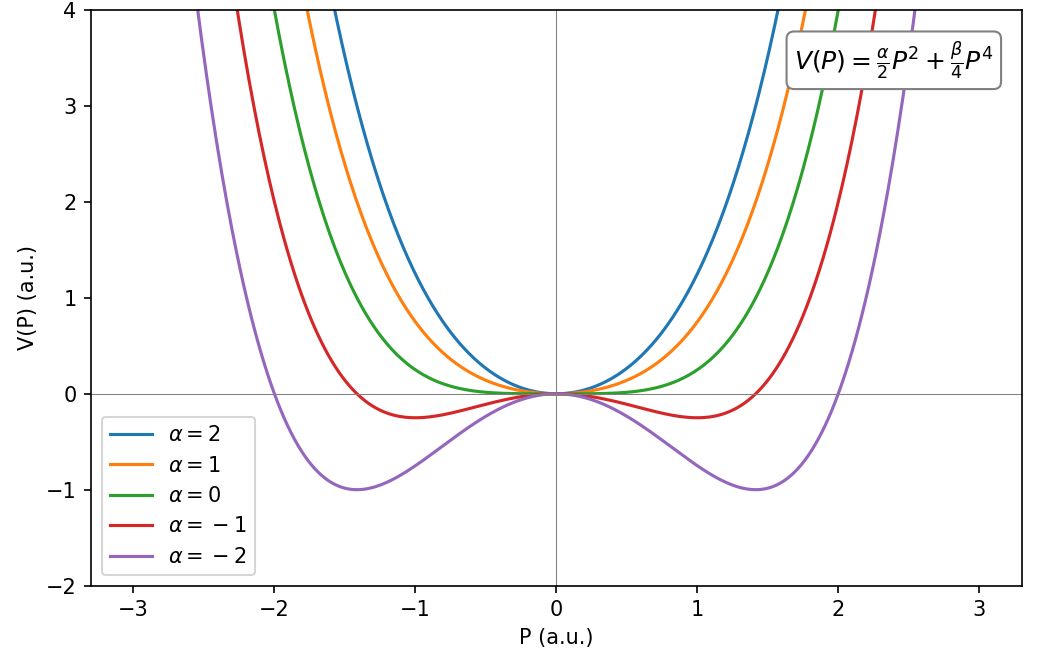
\includegraphics[width=0.78\textwidth]{images/double_puit.png}
\caption{Potentiel local de Landau $V(P)=\alpha P^2/2+\beta P^4/4$ pour
plusieurs valeurs de $\alpha$ (ici $\beta>0$). L'abscisse représente une
composante du paramètre d'ordre local $P(\mathbf x)$ à position fixée ; elle
ne représente pas une dépendance spatiale. Le passage de $\alpha>0$ à
$\alpha<0$ transforme le puits unique paraélectrique en deux minima
ferroélectriques dégénérés. Schéma de l'auteur.}
\label{fig:core_landau_double_well}
\end{figure}

Dans cette représentation, $\alpha$ et $\beta$ sont des coefficients
effectifs et non des constantes microscopiques invariantes. En intégrant, ou en
moyennant, les autres degrés de liberté, les interactions entre modes polaires,
les couplages élastiques et dipolaires, ainsi que les fluctuations thermiques et
quantiques, renormalisent la courbure et les vertices\footnote{En théorie des
champs, un \emph{vertex} désigne le coefficient d'interaction qui relie
plusieurs champs : il est obtenu par dérivées successives du potentiel effectif.
Il peut porter des indices tensoriels ainsi qu'une dépendance en impulsion et en
fréquence.} du potentiel libre. Ils
dépendent donc en pratique de la température, de la pression, de la composition
et de l'échelle de coarse-graining : on devrait écrire
$\alpha_{\rm eff}(T,p,\ldots)$ et $\beta_{\rm eff}(T,p,\ldots)$. Le
changement de signe de $\alpha_{\rm eff}$ est la version la plus simple de
l'adoucissement du mode polaire ; la figure l'illustre en faisant varier
$\alpha$ à $\beta>0$ fixé. Dans un cas plus général, $\beta_{\rm eff}$ est
lui aussi renormalisé et un terme d'ordre six peut devenir nécessaire pour
stabiliser l'énergie libre.

L'analogie du crayon tenu exactement sur sa pointe illustre cette instabilité :
la configuration centrée respecte la symétrie, mais une perturbation
infinitésimale sélectionne l'un des côtés.

\par\medskip
\noindent\textbf{Convention de sommation.}
Dans toute la suite, les indices répétés sont sommés selon la convention
d'Einstein, par exemple
\[
u^\alpha v_\alpha
\equiv\sum_{\alpha=x,y,z}u^\alpha v_\alpha,
\qquad
\eta_\ell B_{\ell m}\eta_m
\equiv\sum_{\ell=1}^{6}\sum_{m=1}^{6}
\eta_\ell B_{\ell m}\eta_m.
\]
Les autres sommes ou intégrales sont écrites explicitement.

\par\medskip
\noindent\textbf{Notation de Voigt.}
La convention de Voigt employée est celle de Vanderbilt--FERAM, avec l'ordre
$(xx,yy,zz,yz,xz,xy)$. Si $\varepsilon_{\alpha\beta}$ désigne le tenseur
symétrique des petites déformations, les vecteurs de déformation et de
contrainte sont
\begin{equation}
\begin{aligned}
\boldsymbol\eta
&=(\varepsilon_{xx},\varepsilon_{yy},\varepsilon_{zz},
2\varepsilon_{yz},2\varepsilon_{xz},2\varepsilon_{xy})^T,\\
\boldsymbol\sigma
&=(\sigma_{xx},\sigma_{yy},\sigma_{zz},
\sigma_{yz},\sigma_{xz},\sigma_{xy})^T.
\end{aligned}
\label{eq:core_voigt_convention}
\end{equation}
Les composantes $4$, $5$ et $6$ de $\boldsymbol\eta$ sont donc les
cisaillements. Les facteurs $2$ ne figurent pas dans le vecteur de
contrainte, de sorte que
$\boldsymbol\sigma^T\boldsymbol\eta
=\sigma_{\alpha\beta}\varepsilon_{\alpha\beta}$.
Enfin, $\mathbf q=(1,1,1,0,0,0)^T$ sélectionne la déformation volumique
$\mathbf q^T\boldsymbol\eta=\operatorname{tr}\boldsymbol\varepsilon$.

\par\medskip
\noindent\textbf{Première zone de Brillouin.}
Un cristal parfait est une structure très symétrique : il peut être essentiellement décrit par la répétition
périodique d'une unité élémentaire ; il n'est donc pas surprenant qu'une description simple équivalente existe en
espace réciproque (ou espace de Fourier/des vecteurs d'ondes).
Pour un réseau cubique primitif de paramètre $a_0$ et de volume
$\Omega_0=a_0^3$, la première zone de Brillouin émerge donc directement de la
périodicité cristalline. Si $\mathbf R$ est un vecteur du réseau de Bravais, le
potentiel microscopique vérifie
\begin{equation}
\begin{aligned}
V(\mathbf r+\mathbf R)&=V(\mathbf r),
&\mathbf R&=\sum_{\nu=1}^{3}n_\nu\mathbf a_\nu,\\
\mathbf a_\mu\!\cdot\!\mathbf b_\nu&=2\pi\delta_{\mu\nu},
&\mathbf G&=\sum_{\nu=1}^{3}m_\nu\mathbf b_\nu,
\end{aligned}
\label{eq:core_direct_reciprocal_lattices}
\end{equation}
où les $\mathbf b_\nu$ engendrent le réseau réciproque. Celui-ci est le support
discret de la transformée de Fourier du réseau direct : la périodicité portée
par les vecteurs $\mathbf R$ se représente dans l'espace de Fourier par les
vecteurs $\mathbf G$. Pour tout site du réseau,
$e^{i\mathbf G\cdot\mathbf R}=1$ ; deux vecteurs d'onde séparés par un
vecteur réciproque décrivent donc la même phase sur les mailles,
\begin{equation}
e^{i(\mathbf k+\mathbf G)\cdot\mathbf R}
=e^{i\mathbf k\cdot\mathbf R},
\qquad \mathbf k\sim\mathbf k+\mathbf G.
\label{eq:core_k_modulo_G}
\end{equation}
On choisit un unique représentant de chaque classe dans la cellule de
Wigner--Seitz du réseau réciproque, appelée première zone de Brillouin :
\begin{equation}
\begin{aligned}
\mathrm{BZ}
&=\left\{\mathbf k:\ |\mathbf k|\leq|\mathbf k-\mathbf G|,
\ \forall\,\mathbf G\neq0\right\}\\
&=\left[-\frac{\pi}{a_0},\frac{\pi}{a_0}\right)^3
\quad\text{pour le réseau cubique simple}.
\end{aligned}
\label{eq:core_first_brillouin_zone}
\end{equation}

\noindent\textbf{Le point $\boldsymbol\Gamma$.}
Le centre de la première zone de Brillouin est appelé point $\Gamma$ :
\begin{equation}
\Gamma\equiv\mathbf k=(0,0,0),
\qquad e^{i\boldsymbol\Gamma\cdot\mathbf R_i}=1
\quad\text{pour toute maille $i$.}
\label{eq:core_gamma_definition}
\end{equation}
Une amplitude de Fourier située à $\Gamma$ possède donc la même phase et la
même valeur dans toutes les mailles. Pour le mode acoustique, elle correspond
à la translation rigide du cristal. Pour le mode polaire optique, elle décrit
au contraire un déplacement relatif uniforme des sous-réseaux ioniques et,
par conséquent, une polarisation macroscopique uniforme. La raideur transverse
du mode polaire au voisinage de $\Gamma$ est ainsi la « masse du mode mou »
qui contrôle la susceptibilité diélectrique homogène.

Développer un noyau « autour de $\Gamma$ » signifie étudier
$\mathbf k=\kappa\widehat{\mathbf n}$ lorsque $\kappa a_0\ll1$, donc des
longueurs d'onde très grandes devant la maille. Pour les interactions
analytiques, la limite $\mathbf k\to0$ rejoint sans ambiguïté la valeur au point
$\Gamma$. Le noyau dipôle--dipôle constitue l'exception importante : son
projecteur $k_\alpha k_\beta/k^2$ dépend de la direction
$\widehat{\mathbf n}$, tandis que la valeur au point exact $\Gamma$ dépend des
conditions électriques macroscopiques aux surfaces. Cette distinction sera
reprise explicitement dans la discussion du noyau dipolaire
(\hyperref[sec:core_dipolar_kernel]{\textcolor{blue}{section~\ref*{sec:core_dipolar_kernel}}}).

La somme directe sur le réseau correspond en espace réciproque à une somme sur les
vecteurs d'onde indépendants, donc dans la première zone de Brillouin.
\phantomsection\label{par:core_sum_to_integral}
La substitution d'une somme par une intégrale est alors naturelle. Pour une
supermaille périodique de côtés $L_x,L_y,L_z$ et de volume
$\Omega=L_xL_yL_z=N\Omega_0$, les vecteurs d'onde autorisés vérifient
\begin{equation}
\begin{aligned}
k_\mu&=\frac{2\pi n_\mu}{L_\mu},
&\Delta k_\mu&=\frac{2\pi}{L_\mu},\\
\Delta^3k&=\prod_{\mu=x,y,z}\Delta k_\mu
=\frac{(2\pi)^3}{\Omega},
&\rho_k&=\frac{1}{\Delta^3k}=\frac{\Omega}{(2\pi)^3},\\
\rho_k\operatorname{Vol}(\mathrm{BZ})
&=\frac{\Omega}{(2\pi)^3}\frac{(2\pi)^3}{\Omega_0}
=\frac{\Omega}{\Omega_0}=N,\\
\sum_{\mathbf k\in\mathrm{BZ}}f(\mathbf k)
&\longrightarrow\frac{\Omega}{(2\pi)^3}
\int_{\mathrm{BZ}}\mathrm d^3k\,f(\mathbf k).
\end{aligned}
\label{eq:core_k_state_density}
\end{equation}
La densité de points $\mathbf k$ croît linéairement avec le volume réel.
Lorsque $\Omega\to\infty$, leur espacement tend vers zéro et la somme devient
une somme de Riemann. La première BZ contient exactement $N$ modes, soit un
mode par maille primitive, et sa frontière constitue la coupure ultraviolette
naturelle héritée du réseau discret.

\subsection{Degrés de liberté et convention de polarisation}

Le modèle associe ainsi à chaque maille $i$ un mode polaire local $u_i^\alpha$
et un déplacement acoustique $w_i^\alpha$. Un mode polaire est, en pratique,
un mode collectif de vibration du réseau. Il est dit polaire parce que les
déplacements relatifs des ions portent une charge effective non nulle et
induisent donc un moment dipolaire, c'est-à-dire une polarisation. Le mode
acoustique décrit au contraire, à grande longueur d'onde, des vibrations pour
lesquelles les atomes se déplacent en phase. À $k=0$, il se réduit à une
translation rigide du cristal ; ses variations spatiales engendrent la
déformation inhomogène.

Avec les conventions du Hamiltonien effectif, le mode polaire produit la
polarisation locale
\begin{equation}
P_i^\alpha=\frac{Z^*}{\Omega_0}u_i^\alpha,
\label{eq:ann_polarisation_locale}
\end{equation}
où $Z^*$ est la charge effective du mode et $\Omega_0$ le volume de la maille de
référence. Cette relation fixe toutes les conversions entre les paramètres
tabulés dans la convention du mode local et ceux utilisés dans la théorie de
champ.

Le mode local est une coordonnée collective : son vecteur propre combine les
déplacements du cation de site A, du titane et des trois oxygènes. Il ne faut
donc pas identifier $u_i$ au déplacement d'un seul ion. La masse effective du
mode et sa charge sont reconstruites à partir du même vecteur propre,
\begin{equation}
M^*=\sum_s M_s\,\lvert\boldsymbol\xi_s\rvert^2,
\qquad
Z^*=\sum_s\boldsymbol\xi_s\mathbin{:}\mathbf Z_s^*,
\label{eq:core_mode_mass_charge}
\end{equation}
ce qui garantit que le terme cinétique et le couplage au champ électrique
emploient la même normalisation.

\begin{figure}[H]
\centering

\includegraphics[width=0.46\textwidth]{mode_local.png}
\caption{Mode local polaire d'une pérovskite cubique. Les flèches donnent les
déplacements relatifs qui composent la coordonnée collective $\mathbf u_i$
~\cite{Zhong1994}.}
\label{fig:core_local_mode}
\end{figure}

\subsection{Hamiltonien discret complet}

Les variables dynamiques sont les trois composantes du mode polaire
$u_i^\alpha$, le déplacement acoustique $w_i^\alpha$ qui génère la déformation
inhomogène, et leurs moments conjugués $\pi_{u,i}^\alpha$ et
$\pi_{w,i}^\alpha$. La déformation homogène
$\eta_\ell^{\rm hom}$ n'est pas un troisième champ dynamique : c'est une
coordonnée mécanique uniforme, sans terme cinétique, dont la valeur est fixée
par l'équilibre thermodynamique sous la contrainte extérieure imposée. Avant
toute limite continue, le modèle employé est
\begin{mdframed}[linecolor=red!60!black,nobreak=true]
\small
\begin{equation}
\begin{aligned}
H_{\rm eff}={}&\sum_i\left[
\frac{\pi_{u,i}^\alpha\pi_{u,i}^\alpha}{2M^*}
+\frac{\pi_{w,i}^\alpha\pi_{w,i}^\alpha}{2M^*_{\rm ac}}
\right]
+\sum_i V_{\rm loc}(\mathbf u_i)\\
&+\frac12\sum_{i\ne j}u_i^\alpha
\big[D_{ij,\alpha\beta}+J_{ij,\alpha\beta}\big]u_j^\beta
+\frac N2\eta_\ell^{\rm hom}\mathcal B_{\ell m}
\eta_m^{\rm hom}\\
&+\frac12\sum_{ij}w_i^\alpha
\Phi^{\rm elas,inh}_{ij,\alpha\beta}w_j^\beta
+\frac12\sum_iB_{\ell\alpha\beta}
\big[\eta_\ell^{\rm hom}+\eta_{i,\ell}^{\rm inh}[w]\big]
u_i^\alpha u_i^\beta
+p\Omega\,q_\ell\eta_\ell^{\rm hom},
\end{aligned}
\label{eq:core_full_discrete_hamiltonian}
\end{equation}
\end{mdframed}
avec $\mathbf q=(1,1,1,0,0,0)^T$ et $\Omega=N\Omega_0$. Le potentiel local
conserve les ordres nécessaires à la stabilité du jeu de paramètres,
\begin{equation}
V_{\rm loc}(\mathbf u)
=\frac12\alpha_0u_\alpha u_\alpha
+\frac14\beta_{\alpha\beta\gamma\delta}
u_\alpha u_\beta u_\gamma u_\delta
+\frac16\gamma_{\alpha\beta\gamma\delta\epsilon\zeta}
u_\alpha\cdots u_\zeta
+\frac18\rho_{\alpha\beta\gamma\delta\epsilon\zeta\eta\theta}
u_\alpha\cdots u_\theta .
\label{eq:core_local_potential_tensor}
\end{equation}
Cette écriture tensorielle compacte doit être reliée aux polynômes scalaires
effectivement tabulés dans les jeux de paramètres
\hyperref[sec:core_parameter_sets]{\textcolor{blue}{(annexe~A)}}.
On note $E_{2n}(\mathbf u)$
la contribution homogène de degré $2n$ en $\mathbf u$, de sorte que
$V_{\rm loc}=E_2+E_4+E_6+E_8$, avec
$E_2=K_2|\mathbf u|^2$ (donc $\alpha_0=2K_2$) et
$E_4=\tfrac14\beta_{\alpha\beta\gamma\delta}
u_\alpha u_\beta u_\gamma u_\delta$. Dans la paramétrisation Nishimatsu, les
deux contributions d'ordre supérieur sont enregistrées directement sous la
forme
\begin{equation}
\begin{aligned}
E_6(\mathbf u)={}&k_1|\mathbf u|^6
+k_2\sum_{\alpha\ne\beta}(u^\alpha)^4(u^\beta)^2
+k_3(u^x)^2(u^y)^2(u^z)^2,\\
E_8(\mathbf u)={}&k_4|\mathbf u|^8.
\end{aligned}
\label{eq:core_cubic_sextic}
\end{equation}
Les $k_1,\ldots,k_4$ sont ici des coefficients anharmoniques locaux et ne
doivent pas être confondus avec les composantes du vecteur d'onde $\mathbf k$.
L'équation~\eqref{eq:core_cubic_sextic} est simplement la forme cubique des
contractions avec les tenseurs $\gamma$ et $\rho$ de
l'équation~\eqref{eq:core_local_potential_tensor}.

\subsection{Élimination de la déformation homogène}

Éliminer la déformation la retire de l'expression finale, tout en conservant son
effet dans les termes induits.
C'est typiquement le mécanisme décrit dans la
\hyperref[sec:core_effective_coefficients]{\textcolor{blue}{section~\ref*{sec:core_effective_coefficients}}} :
les degrés de liberté intégrés ne disparaissent pas physiquement, mais se
traduisent dans les coefficients effectifs de la théorie réduite. Cette
élimination produit précisément le vertex quartique homogène et le contre-terme
quadratique de pression qui seront transformés en espace réciproque. En
notation de Voigt, la contribution homogène s'écrit
\begin{equation}
H_{\mathrm{hom}}(\boldsymbol\eta,\mathbf u;p)
=\frac{N}{2}\boldsymbol\eta^{T}B\boldsymbol\eta
+\boldsymbol\eta^{T}\mathbf g(\mathbf u)
+p\Omega\,\mathbf q^{T}\boldsymbol\eta,
\label{eq:ann_homogene}
\end{equation}
où $B$ est la matrice élastique et $\mathbf g$ le couplage entre déformation et
mode local. Puisque $\boldsymbol\eta$ est une coordonnée uniforme non
dynamique, son équilibre mécanique est obtenu par stationnarité,
\begin{equation}
\boldsymbol\eta^{\star}
=-\frac{1}{N}B^{-1}\!\left[\mathbf g(\mathbf u)
+p\Omega\mathbf q\right].
\label{eq:ann_eta_stationnaire}
\end{equation}
La réinjection de cette solution produit une interaction quartique non locale
entre modes polaires. La contribution ne doit donc pas être confondue avec le
terme quartique local de l'Hamiltonien.

Plus explicitement,
\begin{equation}
g_\ell(\mathbf u)=\frac12\sum_i
B_{\ell\alpha\beta}u_i^\alpha u_i^\beta,
\qquad
\Lambda^{\rm hom}_{\alpha\beta\gamma\delta}
=B_{\ell\alpha\beta}(B^{-1})_{\ell m}B_{m\gamma\delta},
\label{eq:core_g_lambda_hom}
\end{equation}
et la partie indépendante de la déformation devient
\begin{equation}
\begin{aligned}
H_{\rm hom}^{\star}
={}&-\frac{1}{2N}
\big(\mathbf g+p\Omega\mathbf q\big)^TB^{-1}
\big(\mathbf g+p\Omega\mathbf q\big)\\
={}&-\frac{1}{8N}\sum_{ij}
\Lambda^{\rm hom}_{\alpha\beta\gamma\delta}
u_i^\alpha u_i^\beta u_j^\gamma u_j^\delta
+\frac12\sum_i
u_i^\alpha\mathcal P_{\alpha\beta}^{(p,u)}u_i^\beta
+C(p),
\end{aligned}
\label{eq:core_homogeneous_eliminated}
\end{equation}
où le terme constant $C(p)$ n'intervient dans aucune réponse et
\begin{equation}
\mathcal P_{\alpha\beta}^{(p,u)}
=-\frac{p\Omega}{N}\,
q_\ell(B^{-1})_{\ell m}B_{m\alpha\beta}.
\label{eq:core_pressure_kernel_general}
\end{equation}
Pour un cristal cubique, ce tenseur est isotrope :
\begin{equation}
\boxed{
\mathcal P_{\alpha\beta}^{(p,u)}
=-\frac{p\,a_0^3(B_{1xx}+2B_{1yy})}{B_{11}+2B_{12}}\,
\delta_{\alpha\beta}.}
\label{eq:core_pressure_kernel_cubic}
\end{equation}
La pression se projette donc sur la masse du mode mou. Cette identité explique
à la fois sa grande efficacité numérique et le risque d'une mauvaise
interprétation : une « pression effective » ajustée sur $\chi$ est un
contre-terme quadratique, pas une pression mécanique réelle. Cette distinction
est expliquée plus en détail dans la
\hyperref[ann:bto_detail]{\textcolor{blue}{section~\ref*{ann:bto_detail}}}.

Dans la branche cubique centrée, la déformation et la maille reconstruites sont
\begin{equation}
\eta(T,p)=-
\frac{\tfrac12(B_{1xx}+2B_{1yy})\langle u_x^2\rangle+p\,a_0^3}
{B_{11}+2B_{12}},
\qquad
a(T,p)=a_0[1+\eta(T,p)].
\label{eq:core_lattice_reconstruction}
\end{equation}
Cette équation fournit un contrôle indépendant : un protocole de pression peut
être fixé par la maille mesurée, puis utilisé sans réajustement pour prédire la
réponse diélectrique.

\subsection{Conversion locale et conventions de Fourier discrètes}

Sur chaque maille, l'équation~\eqref{eq:ann_polarisation_locale} donne
$u_i^\alpha=sP_i^\alpha$ avec $s=\Omega_0/Z^*$. Il s'agit ici d'un simple
changement local de coordonnée et d'unités, sans passage au continu. Tout
coefficient importé de
l'Hamiltonien de modes locaux doit être multiplié par la puissance correspondante
de $s$ : $s^2$ pour les noyaux quadratiques et la masse, $s^4$ pour les tenseurs
quartiques et les couplages issus des déformations, puis $s^6$ et $s^8$ pour les
termes locaux d'ordre six et huit. Cette comptabilité d'unités est indispensable
pour que la susceptibilité finale soit exprimée dans la convention de
polarisation.

La transformation discrète symétrique est
\begin{equation}
\begin{aligned}
P^\alpha(R_i)&=\frac{1}{\sqrt N}\sum_{k\in\mathrm{BZ}}
\widetilde P^\alpha(k)e^{ik\cdot R_i},
&
\widetilde P^\alpha(k)&=\frac{1}{\sqrt N}\sum_i
P^\alpha(R_i)e^{-ik\cdot R_i}.
\end{aligned}
\label{eq:core_fourier_rules}
\end{equation}
À ce stade, la zone de Brillouin est donc encore un maillage discret de $N$
vecteurs d'onde et ces deux relations constituent un changement de coordonnées
exact et inversible sur le réseau fini.

Après élimination de la coordonnée homogène, l'énergie effective est
décomposée selon
\begin{equation}
H_{\mathrm{eff}}^{\star}
=H_{\mathrm{loc}}+H_{\text{courte portée}}+H_{\mathrm{dip}}
+\Delta H_4^{\mathrm{hom}}+H_{p}^{(2)}
+H_{\mathrm{elas}}^{\mathrm{inh}}+H_{\mathrm{cpl}}^{\mathrm{inh}}+C(p).
\label{eq:ann_decomposition_hamiltonien}
\end{equation}
Les trois premiers termes décrivent le secteur polaire initial ;
$\Delta H_4^{\rm hom}$ et $H_p^{(2)}$ sont respectivement le vertex quartique
et le contre-terme quadratique issus de la déformation homogène. Seul le champ
acoustique associé au secteur inhomogène reste alors à intégrer.

\subsection{Passage terme à terme dans l'espace réciproque}

La normalisation de Fourier est vérifiée avant d'introduire le continu. La
relation d'orthogonalité discrète est
\begin{equation}
\sum_i e^{i(\mathbf k+\mathbf q)\cdot\mathbf R_i}
=N\delta_{\mathbf k,-\mathbf q}.
\label{eq:core_discrete_orthogonality}
\end{equation}
Elle donne, pour le terme local quadratique,
\begin{equation}
\sum_iP_i^\alpha P_i^\beta
=\sum_{\mathbf k}
\widetilde P^\alpha(-\mathbf k)\widetilde P^\beta(\mathbf k),
\label{eq:core_fourier_local_quadratic}
\end{equation}
et, pour n'importe quel noyau de paire invariant par translation,
\begin{equation}
\frac12\sum_{ij}P_i^\alpha
K_{\alpha\beta}(\mathbf R_i-\mathbf R_j)P_j^\beta
=\frac12\sum_{\mathbf k}
\widetilde P^{\alpha *}(\mathbf k)
\widetilde K_{\alpha\beta}(\mathbf k)
\widetilde P^\beta(\mathbf k).
\label{eq:core_fourier_pair_kernel}
\end{equation}
Il ne subsiste donc aucun facteur de $N$ dans le secteur harmonique.

Le terme quartique local conserve en revanche une convolution :
\begin{equation}
\begin{aligned}
\frac14\sum_i\beta_{\alpha\beta\gamma\delta}
P_i^\alpha P_i^\beta P_i^\gamma P_i^\delta
=\frac{1}{4N}\sum_{\mathbf k_1\mathbf k_2\mathbf k_3}
\beta_{\alpha\beta\gamma\delta}\,
\widetilde P^\alpha(\mathbf k_1)
\widetilde P^\beta(\mathbf k_2)
\widetilde P^\gamma(\mathbf k_3)\\
\times\widetilde P^\delta(
-\mathbf k_1-\mathbf k_2-\mathbf k_3).
\end{aligned}
\label{eq:core_fourier_local_quartic}
\end{equation}
Le vertex de déformation homogène porte deux paires de moments opposés,
\begin{equation}
\Delta H_4^{\rm hom}
=-\frac{1}{8N}
\sum_{\mathbf k,\mathbf k'}
\Lambda^{\rm hom}_{\alpha\beta\gamma\delta}
\widetilde P^\alpha(\mathbf k)
\widetilde P^\beta(-\mathbf k)
\widetilde P^\gamma(\mathbf k')
\widetilde P^\delta(-\mathbf k'),
\label{eq:core_fourier_homogeneous_vertex}
\end{equation}
tandis que le couplage acoustique conserve un transfert total
$\mathbf q$ :
\begin{equation}
\widetilde y^{\alpha\beta}(\mathbf q)
=\frac1{\sqrt N}\sum_{\mathbf k}
\widetilde P^\alpha(\mathbf k)
\widetilde P^\beta(\mathbf q-\mathbf k),
\qquad
H_{wP^2}=\frac12\sum_{\mathbf q}
\widetilde w^{\gamma *}(\mathbf q)
\widetilde{\mathcal H}_{\gamma\alpha\beta}(\mathbf q)
\widetilde y^{\alpha\beta}(\mathbf q).
\label{eq:core_fourier_acoustic_convolution}
\end{equation}
Ces quatre identités sont suffisantes pour reconstruire les facteurs de
$N$, les deltas de conservation et toutes les intégrales du Hamiltonien
continu. Le passage thermodynamique
$\sum_{\mathbf k}\to\Omega(2\pi)^{-3}\int_{\rm BZ}\mathrm d^3k$
n'est effectué qu'après cette réduction exacte.

\subsection{Noyau harmonique périodique}

Dans l'espace réciproque, le noyau harmonique complet prend la forme
\begin{equation}
A_{0,\alpha\beta}(k,\omega_n;p)
=m_P\omega_n^2\delta_{\alpha\beta}
+\mathcal P^{(p)}_{\alpha\beta}
+\widetilde D_{\alpha\beta}(k)
+\widetilde J_{\alpha\beta}(k).
\label{eq:ann_noyau_harmonique}
\end{equation}
Le terme dipolaire contient une partie non analytique proportionnelle à
$k_\alpha k_\beta/k^2$. Les intégrations numériques utilisent le noyau
périodique sur toute la zone de Brillouin ; l'expansion à petit
$k$ sert uniquement à interpréter la limite continue à basse énergie.

\subsubsection{Deux niveaux de description : base cubique et noyau périodique}
\label{sec:core_periodic_kernel_descriptions}

La logique de la construction repose sur deux représentations complémentaires,
qu'il ne faut pas confondre. Pour établir la théorie de champ, on ne cherche
d'abord que le comportement de grande longueur d'onde. Le noyau harmonique est
un tenseur cartésien symétrique de rang deux qui doit vérifier, pour toute
opération $R$ du groupe cubique,
\begin{equation}
\Phi(R\mathbf k)=R\,\Phi(\mathbf k)R^T.
\label{eq:core_cubic_covariance_kernel}
\end{equation}
Son développement analytique autour de $\Gamma$, limité au deuxième ordre en
$\mathbf k$, ne peut donc contenir que trois structures quadratiques
indépendantes. En ajoutant la masse cubique et le projecteur dipolaire non
analytique, on obtient la base
\begin{equation}
\begin{aligned}
\Phi_{\alpha\beta}^{(2)}(\mathbf k;p)={}&
A_{0,1}(p)\delta_{\alpha\beta}
+A_{0,2}k^2\delta_{\alpha\beta}
+A_{0,3}k_\alpha k_\beta\\
&+A_{0,4}\delta_{\alpha\beta}k_\alpha^2
+A_{0,5}\frac{k_\alpha k_\beta}{k^2}+O(k^4).
\end{aligned}
\label{eq:core_cubic_rank_two_basis}
\end{equation}
Il n'y a pas de somme sur $\alpha$ dans le terme proportionnel à $A_{0,4}$.
Cette même base est d'abord appliquée au noyau dipôle--dipôle : ses cinq
coefficients sont notés $d_0,\ldots,d_4$. Le noyau analytique de courte portée
fournit séparément $J_0,c_1,c_2,c_3$, tandis que la pression ne contribue qu'au
terme constant. Lors de l'assemblage, les coefficients compatibles avec une
même structure tensorielle s'additionnent pour donner les $A_{0,i}$ ; le
projecteur non analytique $A_{0,5}=d_4$ reste exclusivement dipolaire.
Autrement dit, on décompose un \emph{tenseur de rang deux} sur les structures
autorisées par la symétrie cubique, en ne gardant les termes analytiques que
jusqu'à l'ordre $k^2$. Les deux premières structures quadratiques
$k^2\delta_{\alpha\beta}$ et $k_\alpha k_\beta$ existeraient déjà sous symétrie
de rotation continue ; le terme diagonal
$\delta_{\alpha\beta}k_\alpha^2$ mesure l'anisotropie propre au cristal cubique.
Enfin, $k_\alpha k_\beta/k^2$ n'appartient pas à la série de Taylor : il est
conservé séparément parce qu'il porte la non-analyticité électrostatique et la
séparation LO--TO.

Cette réduction est indispensable pour identifier un petit nombre de
coefficients continus, écrire les termes de gradient de l'action et contrôler
les canaux transverse et longitudinal. Elle est en revanche seulement
asymptotique pour $ka_0\ll1$. Employée jusqu'au bord de la zone de Brillouin,
elle oublierait la périodicité réciproque et les puissances $k^4,k^6,\ldots$
qui codent la physique à l'échelle de la maille.

La récupération ultérieure du code source FERAM a permis de dépasser cette
limitation numérique sans modifier la dérivation de basse énergie. Les
couplages de courte portée sur les 26 voisins et la prescription d'Ewald
permettent de reconstruire directement
\begin{equation}
\Phi_{\rm complet}(\mathbf k;p)
=\Phi^{\rm SR}_{\rm FERAM}(\mathbf k)
+\Phi^{\rm dip}_{\rm Ewald}(\mathbf k)
+\mathcal P^{(p,u)}
\qquad \text{pour tout $\mathbf k\in\mathrm{BZ}$}.
\label{eq:core_full_kernel_hierarchy}
\end{equation}
C'est ce noyau périodique complet qui est envoyé aux quadratures SCHA. Le
développement~\eqref{eq:core_cubic_rank_two_basis} est alors obtenu
\emph{a posteriori} au voisinage de $\Gamma$ et sert à l'interprétation, au
raccord avec la théorie continue et aux tests de cohérence. « Complet » signifie
ici complet au sein du Hamiltonien effectif FERAM et à convergence des sommes
d'Ewald.

\subsubsection{Réduction des tenseurs par symétrie cubique}

La symétrie de la phase cubique constitue un contrôle algébrique avant tout
calcul numérique. Le tenseur quartique complètement symétrique ne contient que
deux invariants :
\begin{equation}
\beta_{\alpha\beta\gamma\delta}
=b_1\big(
\delta_{\alpha\beta}\delta_{\gamma\delta}
+\delta_{\alpha\gamma}\delta_{\beta\delta}
+\delta_{\alpha\delta}\delta_{\beta\gamma}\big)
+b_2\delta_{\alpha\beta\gamma\delta},
\label{eq:core_cubic_quartic}
\end{equation}
où $\delta_{\alpha\beta\gamma\delta}=1$ si les quatre indices sont égaux.
Ainsi
\begin{equation}
\beta_{xxxx}=3b_1+b_2,\qquad
\beta_{xxyy}=\beta_{xyxy}=\beta_{xyyx}=b_1,
\label{eq:core_quartic_components}
\end{equation}
et toute composante contenant un nombre impair d'un indice cartésien est
nulle. Les trois invariants sextiques et l'invariant octique de la
paramétrisation Nishimatsu ont déjà été explicités dans
l'équation~\eqref{eq:core_cubic_sextic}. Ces écritures polynomiales sont
utilisées pour générer les contractions de Wick ; elles évitent de stocker
explicitement des tenseurs de rang six et huit.

\subsubsection{Interaction de courte portée sur les 26 voisins}

Avant de donner sa transformée de Fourier, il faut identifier l'objet réel
qu'elle représente. La partie harmonique locale et de courte portée du
Hamiltonien discret est
\begin{equation}
H_{\rm SR}^{(2)}=
\sum_iK_2u_i^\alpha u_i^\alpha
+\frac12\sum_i\sum_{\mathbf n\in\{-1,0,1\}^3\setminus\{\mathbf0\}}
u_i^\alpha J_{\alpha\beta}(\mathbf n)
u_{i+\mathbf n}^\beta .
\label{eq:core_real_sr_harmonic}
\end{equation}
L'exposant $(2)$ indique que cette énergie est quadratique dans les modes
locaux ; il ne désigne pas une deuxième coquille de voisins. Ici $\mathbf n$
est le vecteur entier sans dimension qui relie deux mailles
séparées par $a_0\mathbf n$, et $J_{\alpha\beta}(\mathbf n)$ est le tenseur de
constantes de force de rang deux qui couple les composantes $\alpha$ et
$\beta$ de leurs modes locaux. La somme contient les six premiers voisins,
les douze deuxièmes voisins et les huit troisièmes voisins ; le facteur
$1/2$ évite de compter deux fois chaque paire.

Ce tenseur n'est pas un tenseur de masse et
l'équation~\eqref{eq:core_real_sr_harmonic} n'est pas une énergie cinétique au
sens temporel. En revanche, son développement à grande longueur d'onde produit
le tenseur de rigidité spatiale
\begin{equation}
G^{\rm SR}_{\alpha\beta\gamma\delta}
=-\frac{a_0^2}{2}\sum_{\mathbf n}
J_{\alpha\beta}(\mathbf n)n_\gamma n_\delta,
\qquad
\mathcal H_{\rm grad}^{\rm SR}
=\frac12G^{\rm SR}_{\alpha\beta\gamma\delta}
(\partial_\gamma P^\alpha)(\partial_\delta P^\beta),
\label{eq:core_real_sr_gradient_tensor}
\end{equation}
dans la densité hamiltonienne continue. Ce terme quadratique en gradients joue
donc, pour les variations dans l'espace, le rôle analogue au terme cinétique
d'une théorie de champ : il pénalise les variations rapides de la
polarisation et fixe la dispersion. La véritable énergie cinétique reste le
terme en $M^*|\dot{\mathbf u}|^2/2$, ou en
$m_P(\partial_\tau\mathbf P)^2/2$ dans l'action euclidienne. La symétrie
cubique réduit $G^{\rm SR}_{\alpha\beta\gamma\delta}$ à trois combinaisons
indépendantes, notées plus bas $G_{11}^{\rm SR}$,
$G_{12}^{\rm SR}$ et $G_{44}^{\rm SR}$.

La transformée de Fourier exacte de
l'équation~\eqref{eq:core_real_sr_harmonic}, et non son développement en
gradients, est la matrice périodique réellement envoyée aux boucles SCHA :
\begin{equation}
\Phi^{\rm SR}_{\alpha\beta}(\mathbf k)
=2K_2\delta_{\alpha\beta}
+\sum_{\mathbf n\in\{-1,0,1\}^3\setminus\{\mathbf0\}}
J_{\alpha\beta}(\mathbf n)
\cos(\mathbf k\cdot a_0\mathbf n).
\label{eq:core_full_sr_kernel}
\end{equation}
Le terme de contact $2K_2\delta_{\alpha\beta}$ est le Hessien de
$K_2|\mathbf u|^2$. L'invariance par inversion,
$J_{\alpha\beta}(\mathbf n)=J_{\alpha\beta}(-\mathbf n)$, explique le cosinus.
Les sept constantes $j_1,\ldots,j_7$ ne sont pas de nouveaux tenseurs : elles
sont les composantes indépendantes de $J_{\alpha\beta}(\mathbf n)$ autorisées
par la symétrie cubique sur les trois coquilles de voisins. Pour les éléments
diagonaux,
\begin{equation}
J_{\alpha\alpha}(\mathbf n)=
\begin{cases}
j_2,&|\mathbf n|^2=1,\ n_\alpha\ne0,\\
j_1,&|\mathbf n|^2=1,\ n_\alpha=0,\\
j_3,&|\mathbf n|^2=2,\ n_\alpha\ne0,\\
j_4,&|\mathbf n|^2=2,\ n_\alpha=0,\\
j_6,&|\mathbf n|^2=3,
\end{cases}
\label{eq:core_sr_diagonal_shells}
\end{equation}
et, si $\alpha\ne\beta$,
\begin{equation}
J_{\alpha\beta}(\mathbf n)=
\begin{cases}
j_5n_\alpha n_\beta,&|\mathbf n|^2=2,\\
j_7n_\alpha n_\beta,&|\mathbf n|^2=3,\\
0,&|\mathbf n|^2=1.
\end{cases}
\label{eq:core_sr_offdiagonal_shells}
\end{equation}
Le développement autour de $\Gamma$ sert uniquement à lire les coefficients
continus :
\begin{equation}
\widetilde J_{\alpha\beta}(\mathbf k)
=J_0\delta_{\alpha\beta}
+c_2k^2\delta_{\alpha\beta}
+2c_3k_\alpha k_\beta
+c_1\delta_{\alpha\beta}k_\alpha^2+O(k^4),
\label{eq:core_sr_small_k}
\end{equation}
avec
\begin{equation}
\begin{aligned}
J_0&=4j_1+2j_2+8j_3+4j_4+8j_6,\\
G_{11}^{\rm SR}&=-a_0^2(j_2+4j_3+4j_6),\\
G_{12}^{\rm SR}&=-4a_0^2(j_5+2j_7),\\
G_{44}^{\rm SR}&=-a_0^2(j_1+2j_3+2j_4+4j_6),\\
c_2&=G_{44}^{\rm SR},\qquad
2c_3=G_{12}^{\rm SR},\qquad
c_1=G_{11}^{\rm SR}-G_{12}^{\rm SR}-G_{44}^{\rm SR}.
\end{aligned}
\label{eq:core_sr_coefficients}
\end{equation}
Prolonger l'équation~\eqref{eq:core_sr_small_k} jusqu'au bord de zone rend
artificiellement instable le point $R$ pour certains jeux de paramètres. Le
solveur emploie donc l'équation~\eqref{eq:core_full_sr_kernel} dans toutes les
intégrales et ne réserve l'expansion qu'à la réponse macroscopique.

\subsubsection{Somme d'Ewald du noyau dipolaire}
\label{sec:core_dipolar_kernel}

Dans la convention du mode local, le tenseur réel entre deux sites distincts
est
\begin{equation}
D_{\alpha\beta}(\mathbf R)
=\frac{Z^{*2}}{\varepsilon_\infty}
\frac{\delta_{\alpha\beta}-3\widehat R_\alpha\widehat R_\beta}{R^3},
\qquad \mathbf R\ne0.
\label{eq:core_real_dipole}
\end{equation}
La somme tridimensionnelle est conditionnellement convergente ; une troncature
directe dépendrait de la forme des coquilles. On introduit donc
$1=\operatorname{erf}(\eta R)+\operatorname{erfc}(\eta R)$. La partie réelle,
absolument convergente, est
\begin{equation}
\begin{aligned}
T_{\alpha\beta}(\mathbf R;\eta)={}&
\frac{\delta_{\alpha\beta}-3\widehat R_\alpha\widehat R_\beta}{R^3}
\left[\operatorname{erfc}(\eta R)
+\frac{2\eta R}{\sqrt\pi}e^{-\eta^2R^2}\right]\\
&-\frac{4\eta^3}{\sqrt\pi}
e^{-\eta^2R^2}\widehat R_\alpha\widehat R_\beta .
\end{aligned}
\label{eq:core_ewald_real_tensor}
\end{equation}
Avec $\mathbf G=2\pi\mathbf m/a_0$, la matrice périodique complète utilisée par
le code vaut
\begin{mdframed}[linecolor=red!60!black,nobreak=true]
\small
\begin{equation}
\begin{aligned}
\Phi^{\rm dip}_{\alpha\beta}(\mathbf k)
=\frac{Z^{*2}}{\varepsilon_\infty}\bigg[
&-\frac{4\eta^3}{3\sqrt\pi}\delta_{\alpha\beta}
+\sum_{\mathbf R\ne0}\cos(\mathbf k\cdot\mathbf R)\,
T_{\alpha\beta}(\mathbf R;\eta)\\
&+\frac{4\pi}{\Omega_0}
\sum_{\mathbf G+\mathbf k\ne0}
\frac{(G_\alpha+k_\alpha)(G_\beta+k_\beta)}
{|\mathbf G+\mathbf k|^2}
\exp\!\left(-\frac{|\mathbf G+\mathbf k|^2}{4\eta^2}\right)
\bigg].
\end{aligned}
\label{eq:core_periodic_ewald_kernel}
\end{equation}
\end{mdframed}
Le premier terme soustrait l'auto-interaction. Le terme réciproque
$\mathbf G=0$ engendre, lorsque $k\to0$, le projecteur longitudinal responsable
de la séparation LO--TO. L'indépendance du résultat vis-à-vis de $\eta$ après
convergence simultanée des deux sommes est un test automatique de
l'implémentation.

Pour relier ce noyau à une théorie de champ, on sépare seulement dans la limite
$k\to0$ :
\begin{equation}
\begin{aligned}
\widetilde D_{\alpha\beta}(\mathbf k)
={}&d_0\delta_{\alpha\beta}
+d_1k^2\delta_{\alpha\beta}
+d_2k_\alpha k_\beta
+d_3\delta_{\alpha\beta}k_\alpha^2
+d_4\frac{k_\alpha k_\beta}{k^2}+O(k^4),\\
d_0={}&-\frac{4\pi Z^{*2}}{3\varepsilon_\infty\Omega_0},
\qquad
d_4=\frac{4\pi Z^{*2}}{\varepsilon_\infty\Omega_0}.
\end{aligned}
\label{eq:core_dipole_small_k}
\end{equation}
Les coefficients $d_{1,2,3}$ sont obtenus en additionnant l'expansion de la
somme réelle, celle des termes $\mathbf G\ne0$ et la correction analytique
$-\pi k_\alpha k_\beta/(\Omega_0\eta^2)$ provenant de l'enveloppe gaussienne
du terme $\mathbf G=0$. Ils ont nécessairement la structure cubique
$k^2\delta_{\alpha\beta}$, $k_\alpha k_\beta$ et
$\delta_{\alpha\beta}k_\alpha^2$.

\subsubsection{Le point \texorpdfstring{$\mathbf k=0$}{k=0} et les conditions de surface}

Il faut distinguer la limite directionnelle $\mathbf k\to0$ du point exact
$\mathbf k=0$. Pour tout $\mathbf k\neq0$, les équations de Maxwell fixent le
projecteur longitudinal $k_\alpha k_\beta/k^2$. Au point $\mathbf k=0$, ce
rapport n'a aucune direction définie : il décrit une polarisation uniforme et
le champ qu'elle produit dépend alors des charges liées
$\sigma_{\rm b}=\overline{\mathbf P}\!\cdot\!\mathbf n$ aux surfaces, de la
forme macroscopique de l'échantillon et des charges libres capables ou non de
les écranter. C'est le contenu physique de la convergence conditionnelle de la
somme dipolaire ; elle ne donne pas une liberté arbitraire, mais oblige à
spécifier une condition électrostatique macroscopique
~\cite{campbell1963existence,BornHuang1954}.

Cette information peut être représentée par un terme de surface
\begin{equation}
\Delta H_{\rm surf}
=\frac{\Omega}{2}\,
\overline P_\alpha\,
\mathcal K^{\rm surf}_{\alpha\beta}\,
\overline P_\beta,
\qquad
\overline{\mathbf P}=\frac1\Omega\int_\Omega\!\mathrm d^3x\,
\mathbf P(\mathbf x),
\label{eq:core_dipole_surface_term}
\end{equation}
où $\mathcal K^{\rm surf}$ contient le tenseur de dépolarisation, le milieu
extérieur et la convention d'ensemble électrique. Pour des électrodes idéales
en court-circuit (ensemble à champ $E$ fixé), les charges libres compensent
les charges liées et $\mathcal K^{\rm surf}=0$ : c'est la convention
« conducteur » ou \emph{tin-foil} de la somme d'Ewald. En circuit ouvert
(ensemble à déplacement $D$ fixé), le champ dépolarisant subsiste ; pour une
plaque uniformément polarisée normalement aux faces, il ajoute au contraire
une raideur longitudinale proportionnelle à
$\mathbf n\mathbf n^T/(\varepsilon_0\varepsilon_\infty)$. Une géométrie
ellipsoïdale générale remplace ce projecteur par son tenseur de
dépolarisation.

Dans le noyau périodique utilisé ici, le vecteur réciproque nul est omis au
point exact $\Gamma$ et aucune correction de surface n'est ajoutée. Le calcul
adopte donc la convention court-circuit ; elle est celle qui correspond à une
mesure diélectrique transverse réalisée entre électrodes sous tension imposée.
Les intégrales utilisent une grille paire ne portant aucun poids sur le point
non analytique. La susceptibilité est extraite de la valeur propre transverse
$A_1=\lim_{\kappa\to0^+}
\mathbf e_T^T A(\kappa\widehat{\mathbf n},0)\mathbf e_T$, avec
$\mathbf e_T\!\cdot\!\widehat{\mathbf n}=0$ ; elle ne dépend donc pas du terme
de dépolarisation longitudinal. Une comparaison à une géométrie ouverte ou à
une réponse longitudinale exigerait en revanche d'ajouter explicitement
l'équation~\eqref{eq:core_dipole_surface_term}.

\subsubsection{Assemblage sans double comptage}

Le noyau harmonique de mode local qui doit être reconstruit pour chaque
$\mathbf k$ est finalement
\begin{equation}
\Phi^{\rm harm}(\mathbf k;p)
=\Phi^{\rm SR}(\mathbf k)+\Phi^{\rm dip}(\mathbf k)
+\mathcal P^{(p,u)},
\qquad
A^{\rm harm}(\mathbf k,\omega_n;p)
=M^*\omega_n^2\mathbb I+\Phi^{\rm harm}(\mathbf k;p).
\label{eq:core_harmonic_assembly}
\end{equation}
À petit $k$, les cinq coefficients ordonnés sont
\begin{equation}
\begin{array}{c|c}
\text{coefficient}&\text{définition}\\ \hline
A_{0,1}&2K_2+J_0+d_0+\mathcal P^{(p,u)}\\
A_{0,2}&c_2+d_1\\
A_{0,3}&2c_3+d_2\\
A_{0,4}&c_1+d_3\\
A_{0,5}&d_4
\end{array}
\label{eq:core_five_coefficients}
\end{equation}
Si $J_0$ ou $d_0$ est absorbé dans une masse locale, il doit disparaître du
noyau explicite. Les deux vérifications distinctes sont
\begin{equation}
\Phi^{\mathrm{harm}}_{\text{périodique}}(\Gamma)
=A_{0,1}\mathbb I,
\qquad
\lim_{\kappa\to0^+}
\Phi^{\mathrm{harm}}(\kappa\widehat{\mathbf n})
=A_{0,1}\mathbb I+A_{0,5}
\widehat{\mathbf n}\widehat{\mathbf n}^{T}.
\label{eq:core_contact_check}
\end{equation}
Le premier contrôle porte sur le contact périodique cubique, le second sur la
séparation transverse--longitudinale. Leur confusion reviendrait précisément à
attribuer au point $\Gamma$ une condition de surface qui n'a pas été choisie.

\subsection{Passage au continu et limite thermodynamique}

Toutes les transformations précédentes sont des identités exactes sur un
réseau fini. Le passage au continu n'est introduit qu'à présent, juste avant la
formulation en termes de champs. Soit $a_0$ le paramètre de maille cubique et
$\Omega_0=a_0^3$. Les règles de correspondance sont
\begin{equation}
\sum_i\longrightarrow\int\frac{\mathrm d^3r}{\Omega_0},
\qquad
u_i^\alpha\longrightarrow u^\alpha(\mathbf r)
=\sqrt{\Omega_0}\,\varphi^\alpha(\mathbf r),
\qquad
P^\alpha(\mathbf r)=\frac{Z^*}{\sqrt{\Omega_0}}\varphi^\alpha(\mathbf r).
\label{eq:core_mapping_rules}
\end{equation}
Cette correspondance réseau--champ ne définit pas, à elle seule, une fonction
précise de classe $C^\infty(\mathbb R^3)$. Attribuer à chaque maille la valeur
moyenne de son mode local produirait un champ constant par morceaux, donc un
champ en escalier. Un champ lisse pourrait être construit par convolution avec
un noyau $K$, par exemple
\[
P_{\rm pc}^\alpha(\mathbf r)
=\sum_iP_i^\alpha\,\mathbf 1_{\mathcal C_i}(\mathbf r),
\qquad
P_K^\alpha(\mathbf r)
=\sum_iP_i^\alpha K(\mathbf r-\mathbf R_i),
\]
où $\mathcal C_i$ est la maille primitive centrée en $\mathbf R_i$. Le choix
du noyau de lissage n'est toutefois pas unique et ne sera pas fixé ici.

Aucune interpolation réelle n'est cependant nécessaire à la théorie
quantique. Les amplitudes de Fourier discrètes ont déjà été introduites par
l'équation~\eqref{eq:core_fourier_rules} au moyen d'un changement de
coordonnées exact et inversible ; chaque $\widetilde P^\alpha(\mathbf k)$ peut
donc être promue directement au rang de coordonnée quantique de mode. Dans la
limite thermodynamique, la seule opération continue requise consiste à
remplacer le maillage réciproque discret par une intégrale sur la première zone
de Brillouin. L'orthogonalité de réseau devient alors une distribution de
Dirac,
\begin{equation}
N\delta_{\mathbf k,-\mathbf q}
\longrightarrow
\frac{(2\pi)^3}{\Omega_0}\,
\delta^{(3)}(\mathbf k+\mathbf q),
\label{eq:core_continuum_orthogonality}
\end{equation}
et la somme sur les vecteurs d'onde vérifie
\begin{equation}
\sum_{\mathbf k\in\mathrm{BZ}}
\longrightarrow
\frac{\Omega}{(2\pi)^3}\int_{\mathrm{BZ}}\mathrm d^3k,
\label{eq:core_sum_to_integral_rule}
\end{equation}
conformément à la densité d'états établie dans le préambule,
équation~\eqref{eq:core_k_state_density}. Cette substitution est physiquement
et mathématiquement justifiée, comme cela est rappelé dans la
\hyperref[par:core_sum_to_integral]{\textcolor{blue}{section~\ref*{sec:origin_dft}
(passage somme--intégrale)}}. Ni noyau de
convolution ni champ continu moyenné physiquement unique ne sont donc
nécessaires. Ces règles suffisent maintenant à écrire l'action euclidienne à
température finie.

\subsection{Action euclidienne à température finie}

Après élimination de la seule coordonnée mécanique homogène, le Hamiltonien
quantique conserve deux champs dynamiques, $\mathbf P$ et $\mathbf w$. À la
température $T$, l'objet statistique fondamental est la fonction de partition
canonique
\begin{equation}
Z=\operatorname{Tr}e^{-\beta\widehat H},
\qquad
\langle\widehat{\mathcal O}\rangle
=\frac{1}{Z}\operatorname{Tr}
\big(\widehat{\mathcal O}e^{-\beta\widehat H}\big),
\qquad \beta=(k_{\rm B}T)^{-1}.
\label{eq:core_partition_trace}
\end{equation}
On insère dans la trace une base complète d'états propres simultanés des
coordonnées de champ,
\begin{equation}
\mathbb I=\int\mathcal D\mathbf P\,\mathcal D\mathbf w\,
|\mathbf P,\mathbf w\rangle\langle\mathbf P,\mathbf w|,
\label{eq:core_field_resolution_identity}
\end{equation}
Après avoir décomposé $e^{-\beta\widehat H}$ en facteurs de temps court, on
insère également entre deux configurations successives la résolution de
l'identité dans la base des moments canoniques
$\boldsymbol\Pi_P$ et $\boldsymbol\Pi_w$ :
\begin{equation}
\begin{aligned}
\mathbb I
&=\int\mathcal D_\hbar\boldsymbol\Pi_P\,
\mathcal D_\hbar\boldsymbol\Pi_w\,
|\boldsymbol\Pi_P,\boldsymbol\Pi_w\rangle
\langle\boldsymbol\Pi_P,\boldsymbol\Pi_w|,\\
\langle\mathbf P,\mathbf w
|\boldsymbol\Pi_P,\boldsymbol\Pi_w\rangle
&=\exp\!\left\{\frac{i}{\hbar}\int_\Omega\!\mathrm d^3x\,
\left[\Pi_P^\alpha P^\alpha+\Pi_w^a w^a\right]\right\},
\end{aligned}
\label{eq:core_momentum_resolution_identity}
\end{equation}
où $\mathcal D_\hbar\boldsymbol\Pi$ désigne, avec le réseau comme
régularisation, le produit des mesures
$\mathrm d\Pi/(2\pi\hbar)$ pour chaque site et chaque composante. Les
commutateurs canoniques ne sont pas choisis arbitrairement : ils réalisent
l'algèbre de Heisenberg associée à toute coordonnée généralisée
$\widehat Q^A$ et à son moment conjugué $\widehat\Pi_B$ :
\[
[\widehat Q^A(\mathbf x),\widehat\Pi_B(\mathbf x')]
=i\hbar\delta^A_{\ B}\delta^{(3)}(\mathbf x-\mathbf x'),
\qquad
[\widehat Q^A,\widehat Q^B]=
[\widehat\Pi_A,\widehat\Pi_B]=0.
\]
Les couples $(\mathbf P,\boldsymbol\Pi_P)$ et
$(\mathbf w,\boldsymbol\Pi_w)$ constituent ici deux copies indépendantes de
cette algèbre.

À chaque tranche de temps, l'exposant contient alors
\begin{equation}
\int_\Omega\!\mathrm d^3x\,
\left[
\frac{\Pi_P^2}{2m_P}+\frac{\Pi_w^2}{2m_w}
-i\boldsymbol\Pi_P\!\cdot\partial_\tau\mathbf P
-i\boldsymbol\Pi_w\!\cdot\partial_\tau\mathbf w
\right].
\label{eq:core_phase_space_short_time}
\end{equation}
L'intégration gaussienne de $\boldsymbol\Pi_P$ et
$\boldsymbol\Pi_w$ produit donc respectivement
$m_P(\partial_\tau\mathbf P)^2/2$ et
$m_w(\partial_\tau\mathbf w)^2/2$. La trace quantique devient ainsi une somme
sur des trajectoires de champs. De manière équivalente, cette construction est obtenue
par analogie avec l'intégrale de chemin de la mécanique quantique et la rotation de Wick
 du temps réel vers le temps imaginaire
$t=-i\tau$. La trace identifie les configurations initiale et finale ; les
champs bosoniques vérifient donc
$\mathbf P(\beta\hbar)=\mathbf P(0)$ et
$\mathbf w(\beta\hbar)=\mathbf w(0)$. Cette dérivation standard à température
finie est présentée en détail par Marino, auquel on pourra se référer au
besoin~\cite[Sec.~5.8]{Marino2017}.

On obtient ainsi l'intégrale de chemin euclidienne
\begin{mdframed}[linecolor=red!60!black,nobreak=true]
\small
\begin{equation}
\begin{aligned}
Z&=\oint_{\text{périodique}}
\mathcal D\mathbf P\,\mathcal D\mathbf w\;
e^{-\mathcal S_E[\mathbf P,\mathbf w]/\hbar},\\
\mathcal S_E[\mathbf P,\mathbf w]
&=\int_0^{\beta\hbar}\!\mathrm d\tau
\left\{
\int_\Omega\!\mathrm d^3x\,
\left[\frac{m_P}{2}(\partial_\tau P^\alpha)^2
+\frac{m_w}{2}(\partial_\tau w^a)^2\right]
+H_{\rm pot}^{\star}[\mathbf P,\mathbf w;p]
\right\}.
\end{aligned}
\label{eq:core_quantum_action}
\end{equation}
\end{mdframed}
L'étoile rappelle que $\boldsymbol\eta^{\rm hom}$ a déjà été remplacée par sa
valeur stationnaire. En revanche, $\mathbf w(\mathbf x,\tau)$ reste à ce stade
un champ intégré sur toutes ses trajectoires : l'élimination de la déformation
inhomogène requiert l'évaluation de l'intégrale gaussienne.
Dans la limite semi-classique, l'intégrale
fonctionnelle s'évalue par la méthode de Laplace, ou approximation du
point selle. Les configurations stationnaires satisfaisant
$\delta\mathcal S_E/\delta\mathbf P=
\delta\mathcal S_E/\delta\mathbf w=0$ dominent. Une trajectoire dont l'action excède
celle du point selle de $\Delta\mathcal S_E>0$ est supprimée par le facteur
$e^{-\Delta\mathcal S_E/\hbar}$.

La périodicité sur l'intervalle de longueur $\beta\hbar$ impose les fréquences
bosoniques de Matsubara. Pour $X= P$ ou $w$,
\begin{equation}
X^a(\mathbf x,\tau)
=\frac{1}{\sqrt{\beta\hbar}}\sum_{n\in\mathbb Z}
\widetilde X^a(\mathbf x,\omega_n)e^{-i\omega_n\tau},
\qquad
\omega_n=\frac{2\pi n}{\beta\hbar}.
\label{eq:core_matsubara_transform}
\end{equation}
Dans l'espace de Fourier--Matsubara, la structure de l'action avant intégration
du mode acoustique est donc
\begin{equation}
\begin{aligned}
\mathcal S_E={}&
\frac12\sum_K\widetilde P^{\alpha *}(K)
A^{(P)}_{0,\alpha\beta}(K;p)\widetilde P^\beta(K)\\
&+\frac12\sum_K\widetilde w^{a*}(K)
A^{(w)}_{ab}(K)\widetilde w^b(K)
+\mathcal S_{\rm anh}[P]+\mathcal S_{wP^2}[P,w].
\end{aligned}
\label{eq:core_action_two_fields}
\end{equation}
où $K=(\mathbf k,\omega_n)$ et $\sum_K$ inclut la somme de Matsubara et
l'intégrale sur la première zone de Brillouin. Le noyau polaire nu combine la
dynamique $m_P\omega_n^2$, les coefficients locaux, le contre-terme de pression,
le tenseur de courte portée périodique et le noyau dipolaire non analytique.

\subsection{Intégration du mode acoustique et déformation inhomogène}

L'élimination du secteur inhomogène est maintenant effectuée au niveau de
l'action. La déformation inhomogène n'est pas une variable fonctionnelle supplémentaire :
elle est la dérivée spatiale du champ acoustique. Sur la maille réciproque de
FERAM,
\begin{equation}
\boldsymbol\eta^{\rm inh}(\mathbf k)
=\mathcal L(\mathbf k)\mathbf w(\mathbf k),
\qquad
\mathcal L(\mathbf k)=
\begin{pmatrix}
k_x&0&0\\
0&k_y&0\\
0&0&k_z\\
0&k_z&k_y\\
k_z&0&k_x\\
k_y&k_x&0
\end{pmatrix},
\qquad
\mathcal H_{s\alpha\beta}=\mathcal L_{\ell s}B_{\ell\alpha\beta}.
\label{eq:core_feram_strain_operator}
\end{equation}
La phase $i$ associée à $\partial_\alpha\mapsto ik_\alpha$ disparaît dans
$\mathcal H^\dagger G_w\mathcal H$.

Le champ acoustique est couplé au champ quadratique local
\begin{equation}
\widetilde y^{bc}(q,\omega_n)
=\frac{1}{\sqrt{N\beta\hbar}}\sum_m
\frac{\Omega}{(2\pi)^3}\int_{\mathrm{BZ}}\!\mathrm d^3k\;
\widetilde P^b(k,\omega_m)
\widetilde P^c(q-k,\omega_n-\omega_m).
\label{eq:core_y_quadratic}
\end{equation}
Pour employer dès cette étape la même mesure intensive que dans les boucles
SCHA, posons
\begin{equation}
Q\equiv(\mathbf q,\omega_n),\qquad
\int_Q\equiv
\frac{1}{\beta}\sum_{n\in\mathbb Z}
\frac{\Omega_0}{(2\pi)^3}\int_{\rm BZ}\!\mathrm d^3q,
\qquad
\int_{Q_1,\ldots,Q_r}\equiv\prod_{j=1}^{r}\int_{Q_j}.
\label{eq:core_compact_Q_measure}
\end{equation}
Comme $\Omega=N\Omega_0$, la somme extensive antérieurement notée $\sum_Q$
vaut $N\beta\int_Q$.
Sa partie de l'action s'écrit, avec une combinaison explicitement réelle,
\begin{equation}
\begin{aligned}
\mathcal S_w
=N\beta\int_Q\left[
\frac12\widetilde w^{a*}A^{(w)}_{ab}\widetilde w^b
+\frac14\left(\widetilde w^{a*}F_a+F_a^*\widetilde w^a\right)
\right],\\
A^{(w)}_{ab}(Q)=m_w\omega_n^2\delta_{ab}
+\widetilde\Phi^{\mathrm{elas,inh}}_{ab}(q),
\qquad
F_a(Q)=\widetilde{\mathcal H}_{abc}(q)\widetilde y^{bc}(Q),
\end{aligned}
\label{eq:core_acoustic_action}
\end{equation}
En posant $G_w=[A^{(w)}]^{-1}$, la complétion du carré donne
\begin{equation}
\widetilde w_\star^a=-\frac12G_w^{ad}F_d,
\qquad
\Delta\mathcal S_{\mathrm{inh}}[P]
=-\frac{N\beta}{8}\int_Q
\widetilde y^{bc*}(Q)\,
\mathcal M^{\mathrm{inh}}_{bc,ef}(Q)\,
\widetilde y^{ef}(Q),
\label{eq:core_inhomogeneous_elimination}
\end{equation}
avec
\begin{equation}
\mathcal M^{\mathrm{inh}}_{bc,ef}(Q)
=\widetilde{\mathcal H}^{*}_{abc}(q)
G_w^{ad}(Q)\widetilde{\mathcal H}_{def}(q).
\label{eq:core_inhomogeneous_vertex}
\end{equation}
Dans la phase cubique centrosymétrique, l'inversion spatiale impose
$A^{(w)}(\mathbf q,\omega_n)=A^{(w)}(-\mathbf q,\omega_n)$ ; la dépendance
en $\omega_n^2$ rend également ce noyau pair en fréquence. Ainsi
$G_w(-Q)=G_w(Q)$. Comme
$\mathcal L(-\mathbf q)=-\mathcal L(\mathbf q)$, on a aussi
$\widetilde{\mathcal H}(-\mathbf q)=-\widetilde{\mathcal H}(\mathbf q)$,
et la définition précédente entraîne
\begin{equation}
\mathcal M^{\rm inh}_{bc,ef}(-Q)=\mathcal M^{\rm inh}_{bc,ef}(Q),
\qquad
\mathcal M^{\rm inh}_{bc,ef}
=\mathcal M^{\rm inh}_{cb,ef}
=\mathcal M^{\rm inh}_{bc,fe}.
\label{eq:core_inhomogeneous_vertex_parity}
\end{equation}
Les dernières symétries, dites mineures, suivent de
$B_{\ell\alpha\beta}=B_{\ell\beta\alpha}$. De même, le noyau polaire
centrosymétrique vérifie
$A_{ab}(\mathbf k,\omega_n)=A_{ab}(-\mathbf k,\omega_n)$ et, puisque sa
dynamique est paire en $\omega_n$, $A(K)=A(-K)$.
Il ne s'agit pas ici de remplacer prématurément $\mathbf w$ par une
configuration statique. Puisque $\mathcal S_w$ est quadratique en $\mathbf w$,
l'intégrale fonctionnelle est gaussienne et exacte :
\begin{equation}
\int\mathcal D\mathbf w\,e^{-\mathcal S_w/\hbar}
\propto[\det A^{(w)}]^{-1/2}
e^{-\Delta\mathcal S_{\rm inh}[P]/\hbar}.
\label{eq:core_acoustic_gaussian_integral}
\end{equation}
Le déterminant, indépendant de $P$ dans ce modèle harmonique acoustique, ne
modifie pas les équations polaires.

Cette intégration conserve la dépendance en impulsion et en fréquence du
vertex quartique médié par les phonons acoustiques. Les trois interactions
$\beta$, $\Lambda^{\rm hom}$ et $\mathcal M^{\rm inh}$ restent donc séparées
dans la fermeture auto-cohérente.

% =============================================================================
\section{Fermeture harmonique auto-cohérente et réponse diélectrique}
\label{ann:scha_reponse}
% =============================================================================

Les termes d'ordre supérieur à deux empêchent d'évaluer l'intégrale
fonctionnelle par une simple intégration gaussienne : la fonction de partition
reste bien définie formellement, mais elle n'est plus calculable analytiquement
par complétion du carré. La SCHA fournit une fermeture calculable en remplaçant
la dynamique anharmonique par celle d'un Hamiltonien harmonique effectif,
optimisé séparément à chaque température.

Cette stratégie est particulièrement motivée pour SrTiO$_3$. Les calculs de
phonons auto-cohérents de Tadano et Tsuneyuki reproduisent la stabilisation et
l'évolution thermique des phonons anharmoniques du cristal cubique
SrTiO$_3$~\cite{TadanoTsuneyuki2015}.

La SCHA retenue est non perturbative, car le noyau renormalisé entre dans sa
propre covariance, mais elle n'est pas exacte : l'optimisation reste restreinte
à une famille de mesures gaussiennes et n'explicite ni les cumulants connexes
d'ordre supérieur à deux ni les corrections dynamiques non gaussiennes. Cette
limite motive le diagnostic post-SCHA
(\hyperref[ann:post_scha_fr]{\textcolor{blue}{section~\ref*{ann:post_scha_fr}}}) :
si une correction de volume et un
potentiel microscopique enrichi ne rétablissent pas la réponse, tandis que la
dynamique moléculaire fondée sur ce potentiel en retrouve la tendance,
l'hypothèse gaussienne devient un goulot d'étranglement plausible. Le test
consiste alors à vérifier que la première auto-énergie non gaussienne assouplit
la réponse dans le sens attendu tout en restant petite devant le noyau SCHA.

La méthode auto-cohérente peut être mise en parallèle avec les diagrammes de
Feynman. Dans cette représentation, une ligne interne est le propagateur
$D=A^{-1}$, un vertex représente un couplage anharmonique du potentiel et une
boucle est une intégration interne $\int_QD_Q$. Pour un vertex quartique, la
contraction d'une paire de jambes forme l'auto-énergie locale de Hartree,
notée schématiquement $\Sigma_{\rm H}[D]$. L'équation
\begin{equation}
A=A_0+\Sigma_{\rm H}[D],
\qquad D=A^{-1},
\label{eq:core_hartree_diagrammatic_closure}
\end{equation}
est alors auto-cohérente : la boucle qui corrige le noyau est elle-même
calculée avec le propagateur corrigé. La résolution du point fixe resomme ainsi
la famille infinie des diagrammes de Hartree dits \emph{daisy} et
\emph{superdaisy}. Elle ne constitue pas la somme de tous les diagrammes : les
corrections irréductibles à deux points, telles que le diagramme \emph{sunset},
portent une dépendance supplémentaire en impulsion et en fréquence et sont
examinées séparément dans le diagnostic post-SCHA
(\hyperref[ann:post_scha_fr]{\textcolor{blue}{section~\ref*{ann:post_scha_fr}}}).

\begin{figure}[htbp]
\centering
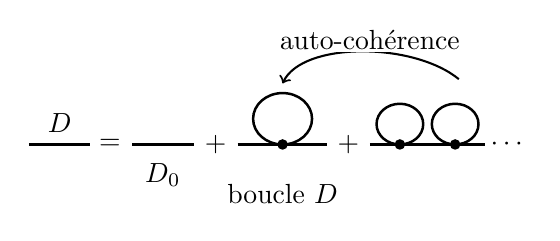
\begin{tikzpicture}[x=0.78cm,y=0.68cm,
  propagator/.style={draw=black,line width=0.9pt},
  vertex/.style={fill=black,circle,inner sep=1.35pt}]
  \draw[propagator] (0,0) -- (1.00,0);
  \node[above] at (0.50,0.04) {$D$};
  \node at (1.32,0) {$=$};
  \draw[propagator] (1.68,0) -- (2.68,0);
  \node[below] at (2.18,-0.18) {$D_0$};
  \node at (3.04,0) {$+$};
  \draw[propagator] (3.40,0) -- (4.86,0);
  \node[vertex] at (4.13,0) {};
  \draw[propagator] (4.13,0.48) circle (0.48);
  \node[below] at (4.13,-0.56) {boucle $D$};
  \node at (5.20,0) {$+$};
  \draw[propagator] (5.55,0) -- (7.42,0);
  \node[vertex] at (6.04,0) {};
  \node[vertex] at (6.94,0) {};
  \draw[propagator] (6.04,0.38) circle (0.38);
  \draw[propagator] (6.94,0.38) circle (0.38);
  \node at (7.78,0) {$\cdots$};
  \draw[->,line width=0.75pt] (7.00,1.22)
    .. controls (6.25,1.92) and (4.45,1.92) .. (4.13,1.14);
  \node[fill=white,inner sep=1pt] at (5.55,1.95) {auto-cohérence};
\end{tikzpicture}
\caption{Représentation diagrammatique de la fermeture de Hartree : une
insertion quartique et sa boucle interne corrigent le propagateur ; le
propagateur corrigé est réinjecté dans cette même boucle. La solution
auto-cohérente resomme la suite des contributions \emph{daisy} et
\emph{superdaisy}. Schéma de l'auteur.}
\label{fig:core_hartree_daisy}
\end{figure}


\subsection{Principe variationnel et contenu de l'approximation}
\label{sec:core_scha_variational_principle}

À température $T$ fixée, le potentiel anharmonique n'est pas conservé dans
l'Hamiltonien d'essai : il est remplacé par le potentiel quadratique
$V_A=\tfrac12\mathbf P\cdot A\cdot\mathbf P$. Le vrai potentiel $V$ reste
néanmoins présent dans la fonctionnelle variationnelle, uniquement à travers
la moyenne du reste $V-V_A$ qui sert à sélectionner le noyau optimal. On
considère ainsi la famille d'Hamiltoniens harmoniques centrés $H_A[A]$,
paramétrée uniquement par un noyau positif $A$. C'est cette branche
paraélectrique centrée qui est utilisée dans tous les calculs numériques du
présent travail.

Les Hamiltoniens exact et d'essai possèdent le même terme cinétique :
$H=T_{\rm cin}+V[\mathbf P]$ et $H_A=T_{\rm cin}+V_A[\mathbf P]$. Leur
différence ne contient donc plus le terme cinétique :
$H-H_A=V-V_A$. Avant d'introduire la fonctionnelle variationnelle, rappelons
les deux niveaux auxquels ce noyau intervient. Sur le réseau, le noyau nu
complet, périodique sur toute la zone de Brillouin et exprimé dans la
convention du déplacement local $u$, est
\begin{equation}
\boxed{
A^{(u)}_{0,\alpha\beta}(\mathbf k,\omega_n;p)
=M^*\omega_n^2\delta_{\alpha\beta}
+\Phi^{\rm SR}_{\alpha\beta}(\mathbf k)
+\Phi^{\rm dip,Ewald}_{\alpha\beta}(\mathbf k)
+\mathcal P^{(p,u)}_{\alpha\beta}.}
\label{eq:core_scha_full_bare_kernel}
\end{equation}

La somme dipolaire d'Ewald se décompose, au voisinage de $\Gamma$, en une
partie analytique et une partie non analytique, cette dernière portant le
projecteur longitudinal responsable de la séparation LO--TO. Le développement
de basse énergie associé à l'équation~\eqref{eq:core_scha_full_bare_kernel} est
alors précisément la base cubique de l'équation~\eqref{eq:core_cubic_rank_two_basis} :
\begin{equation}
\begin{aligned}
A^{(u),\rm LE}_{0,\alpha\beta}(\mathbf k,\omega_n;p)
={}&M^*\omega_n^2\delta_{\alpha\beta}
+A^{(u)}_{0,1}(p)\delta_{\alpha\beta}
+A^{(u)}_{0,2}k^2\delta_{\alpha\beta}
+A^{(u)}_{0,3}k_\alpha k_\beta\\
&+A^{(u)}_{0,4}\delta_{\alpha\beta}k_\alpha^2
+A^{(u)}_{0,5}\frac{k_\alpha k_\beta}{k^2}+O(k^4).
\end{aligned}
\label{eq:core_scha_low_energy_kernel}
\end{equation}
Ce second noyau suffit pour identifier la masse transverse du mode mou,
$A_1^{(u)}=\lim_{\kappa\to0^+}\mathbf e_T^T
A^{(u)}(\kappa\widehat{\mathbf n},0)\mathbf e_T$, et donc la réponse uniforme
$\chi_T\propto \big(A_1^{(u)}\big)^{-1}$. Il ne doit toutefois pas être prolongé
artificiellement jusqu'au bord de zone : les boucles SCHA intègrent tous les
moments $\mathbf k\in\mathrm{BZ}$ et requièrent le noyau périodique complet,
comme expliqué en
\hyperref[sec:core_periodic_kernel_descriptions]{\textcolor{blue}{section~\ref*{sec:core_periodic_kernel_descriptions}}}.
Dans la fermeture cubique, la masse est calibrée par sa projection transverse
au centre de zone, mais l'ansatz déplace cette masse de manière isotrope dans
l'espace cartésien. La seule inconnue est ainsi l'amplitude scalaire de ce
décalage ; l'équation optimisée n'est pas une équation matricielle complète.
Cette réduction ne vaut plus, en général, dans la phase ferroélectrique, où la
symétrie cubique est brisée et où des composantes transverse et longitudinale
peuvent devoir être renormalisées séparément.
L'équation SCHA correspondante en phase ferroélectrique, dans laquelle le
centroïde et le noyau harmonique doivent être déterminés conjointement, est
dérivée formellement dans
l'\hyperref[sec:core_ferroelectric_extension]{\textcolor{blue}{annexe~\ref*{sec:core_ferroelectric_extension}}}.
Cette extension précise le cadre théorique, mais n'est pas résolue
numériquement dans ce rapport.
\begin{equation}
A^{(u)}(Q;A_1^{(u)})=M^*\omega_n^2\mathbb I
+\Phi^{\rm SR}(\mathbf k)+\Phi^{\rm dip,Ewald}(\mathbf k)
+\mathcal P^{(p,u)}
+\big[A_1^{(u)}-A^{(u)}_{0,1}(p)\big]\mathbb I.
\label{eq:core_full_lattice_trial_kernel}
\end{equation}
Ainsi, la limite de basse énergie interprète la susceptibilité à $k=0$, tandis
que la somme complète d'Ewald et les couplages de courte portée sur réseau
contrôlent quantitativement les contractions internes. Pour revenir au champ
$P=u/s$, avec $s=\Omega_0/Z^*$, on applique
\begin{equation}
A^{(P)}=s^2A^{(u)},\qquad A_1^{(P)}=s^2A_1^{(u)},\qquad
m_P=s^2M^*,\qquad G^{(P)}=s^{-2}G^{(u)}.
\label{eq:core_scha_u_p_conversion}
\end{equation}
Les tenseurs d'ordre $2n$ sont multipliés par $s^{2n}$. Dans les équations
variationnelles qui suivent, $A$, $A_0$, $A_1$, les vertex et la covariance
$G$ sont tous exprimés dans la convention $P$ ; en particulier
$A_1\equiv A_1^{(P)}$. Dans une énergie potentielle, $A$ désigne sa partie
statique ; le terme cinétique commun est ajouté dans l'action de Matsubara.
La borne de Gibbs--Bogoliubov s'écrit donc ici directement
\begin{equation}
\begin{gathered}
F\leq F_{\rm var}[A;T]
=F_A[A;T]
+\left\langle
V[\mathbf P]-V_A[\mathbf P]
\right\rangle_A,
\qquad
V_A[\mathbf P]
=\frac12\,\mathbf P\mathbin{\cdot}A
\mathbin{\cdot}\mathbf P,\\
A_\star(T)=\underset{A>0}{\operatorname{arg\,min}}\;
F_{\rm var}[A;T].
\end{gathered}
\label{eq:core_gibbs_bogoliubov}
\end{equation}
Le noyau optimal ne minimise donc pas
séparément $\langle V-V_A\rangle_A$ : il minimise la somme de ce reste moyen et
de $F_A[A;T]$. C'est en ce sens précis que la SCHA recherche, à température
fixée, la meilleure approximation harmonique du vrai potentiel.

La logique de la fermeture peut être résumée schématiquement par
\begin{equation}
A_0(K)+V_{\rm anh}[\mathbf P]
\xrightarrow[\text{à température }T]{\mathrm{SCHA}}
A(K;T).
\label{eq:core_scha_mapping}
\end{equation}


\subsection{Action d'essai}

Pour construire la mesure $\langle\cdot\rangle_A$, la SCHA introduit l'action
gaussienne d'essai, avec la transformée temporelle symétrique de
l'équation~\eqref{eq:core_matsubara_transform} et le poids $e^{-\mathcal S_0/\hbar}$,
\begin{equation}
\mathcal S_0
=\frac12
\sum_n\frac{\Omega}{(2\pi)^3}\int_{\mathrm{BZ}}\!\mathrm d^3k\,
p^\alpha(-k,-\omega_n)
A_{\alpha\beta}(k,\omega_n;T)
p^\beta(k,\omega_n).
\label{eq:ann_action_essai}
\end{equation}
Le noyau $A$ est déterminé par la stationnarité de la borne variationnelle de
Gibbs--Bogoliubov. La covariance gaussienne est
\begin{equation}
\left\langle
p^\alpha(k,\omega_n)p^\beta(k',\omega_m)
\right\rangle_0
=\hbar\,\frac{(2\pi)^3}{\Omega}
\delta^{(3)}(k+k')\delta_{n,-m}
\left[A^{-1}(k,\omega_n;T)\right]^{\alpha\beta}.
\label{eq:ann_covariance}
\end{equation}

Pour rendre explicite le passage entre la moyenne gaussienne et l'équation
auto-cohérente sans alourdir chaque ligne, on utilise la mesure $\int_Q$
introduite avant l'équation~\eqref{eq:core_acoustic_action}, en renommant sa
variable muette $\mathbf q$ en $\mathbf k$ lorsque cela est commode, ainsi que
\begin{equation}
D_Q^{\alpha\beta}\equiv
\left[A^{-1}(\mathbf k,\omega_n;T)\right]^{\alpha\beta},
\qquad
\int_{\mathbf k;n,n'}\equiv
\frac{1}{\beta^2}\sum_{n,n'}
\frac{\Omega_0}{(2\pi)^3}\int_{\rm BZ}\!\mathrm d^3k.
\label{eq:core_compact_propagator_notation}
\end{equation}
Le facteur $\Omega_0$ normalise l'intégrale par maille primitive. En notant
$f=F/N$, le théorème de Wick appliqué à
$f_{\rm var}=f_A+N^{-1}\langle V-V_A\rangle_A$\footnote{Pour une mesure
gaussienne centrée, les moments impairs sont nuls et
\(\langle\xi_{a_1}\cdots\xi_{a_{2n}}\rangle
=\sum_{\mathcal P}\prod_{(i,j)\in\mathcal P}
\langle\xi_{a_i}\xi_{a_j}\rangle\), où la somme porte sur les
\((2n-1)!!\) appariements des \(2n\) champs.} donne alors la forme
développée compacte
\begin{equation}
\begin{aligned}
f_{\rm var}-f_A={}&
\frac12\int_Q(A_{0,Q}-A_Q)_{\alpha\beta}D_Q^{\alpha\beta}\\
&+\frac14\beta_{\alpha\beta\gamma\delta}
\int_{Q,Q'}\!\Big(
D_Q^{\alpha\beta}D_{Q'}^{\gamma\delta}
+D_Q^{\alpha\gamma}D_{Q'}^{\beta\delta}
+D_Q^{\alpha\delta}D_{Q'}^{\beta\gamma}\Big)\\
&-\frac18\Lambda^{\rm hom}_{\alpha\beta\gamma\delta}
\int_{Q,Q'}D_Q^{\alpha\beta}D_{Q'}^{\gamma\delta}\\
&-\frac{1}{4N}\int_{\mathbf k;n,n'}
\Lambda^{\rm hom}_{\alpha\gamma\beta\delta}
D_{(-\mathbf k,\omega_n)}^{\alpha\beta}
D_{(\mathbf k,\omega_{n'})}^{\gamma\delta}\\
&-\frac14\int_{Q,Q'}
\mathcal M^{\rm inh}_{\alpha\gamma,\beta\delta}(Q-Q')
D_Q^{\alpha\beta}D_{Q'}^{\gamma\delta}\\
&+\frac16\gamma_{\alpha\beta\gamma\delta\epsilon\zeta}
\int_{Q,Q',Q''}\!\Big[
D_Q^{\alpha\beta}D_{Q'}^{\gamma\delta}D_{Q''}^{\epsilon\zeta}
+\text{14 autres appariements}\Big]\\
&+\frac18\rho_{\alpha\beta\gamma\delta\epsilon\zeta\eta\theta}
\int_{Q,Q',Q'',Q'''}\!\Big[
D_Q^{\alpha\beta}D_{Q'}^{\gamma\delta}
D_{Q''}^{\epsilon\zeta}D_{Q'''}^{\eta\theta}
+\text{104 autres appariements}\Big] .
\end{aligned}
\label{eq:core_variational_wick_expanded}
\end{equation}
La première ligne est exactement la contraction de la différence entre le
potentiel quadratique nu et le potentiel d'essai,
$\tfrac12\mathbf P\mathbin{\cdot}(A_0-A)\mathbin{\cdot}\mathbf P$ ; toutes les
lignes suivantes proviennent des interactions quartiques, sextiques et
octiques conservées dans $V$.
Les sommes d'appariements portent à la fois sur les indices tensoriels et sur
les arguments $Q,Q',\ldots$ correspondants. Le terme homogène proportionnel à
$1/N$ est écrit pour conserver la dérivation complète ; il disparaît dans la
densité d'énergie libre à la limite thermodynamique.

La boucle locale, est maintenant définie par
\begin{equation}
G^{\mu\nu}(T)\equiv\int_QD_Q^{\mu\nu}
=\left\langle
\delta P^\mu(\mathbf r,\tau)\delta P^\nu(\mathbf r,\tau)
\right\rangle_0 .
\label{eq:core_equal_point_covariance}
\end{equation}
Elle est intensive et normalisée par maille. La contraction non locale issue
de l'élimination du mode acoustique est, de même,
\begin{equation}
\mathcal I^{\rm inh}_{\alpha\beta}(K;A)
\equiv\int_Q
\mathcal M^{\rm inh}_{\alpha\gamma,\beta\delta}(K-Q)
D_Q^{\gamma\delta}.
\label{eq:core_inhomogeneous_self_energy}
\end{equation}
Cette convolution est l'insertion d'auto-énergie engendrée par l'élimination
de la déformation inhomogène.
Avec ces deux définitions, la même énergie libre variationnelle se réécrit
\begin{equation}
\begin{aligned}
f_{\rm var}[A;T]={}&f_A[A;T]
+\frac12\int_Q(A_{0,Q}-A_Q)_{\alpha\beta}D_Q^{\alpha\beta}\\
&+\frac14\beta_{\alpha\beta\gamma\delta}
\big(G^{\alpha\beta}G^{\gamma\delta}
+G^{\alpha\gamma}G^{\beta\delta}
+G^{\alpha\delta}G^{\beta\gamma}\big)\\
&-\frac18\Lambda^{\rm hom}_{\alpha\beta\gamma\delta}
G^{\alpha\beta}G^{\gamma\delta}
-\frac{1}{4N}\int_{\mathbf k;n,n'}
\Lambda^{\rm hom}_{\alpha\gamma\beta\delta}
D_{(-\mathbf k,\omega_n)}^{\alpha\beta}
D_{(\mathbf k,\omega_{n'})}^{\gamma\delta}\\
&-\frac14\int_Q
D_Q^{\alpha\beta}\mathcal I^{\rm inh}_{\alpha\beta}(Q;A)\\
&+\frac16\gamma_{\alpha\beta\gamma\delta\epsilon\zeta}
\Big[G^{\alpha\beta}G^{\gamma\delta}G^{\epsilon\zeta}
+\text{14 autres appariements}\Big]\\
&+\frac18\rho_{\alpha\beta\gamma\delta\epsilon\zeta\eta\theta}
\Big[G^{\alpha\beta}G^{\gamma\delta}
G^{\epsilon\zeta}G^{\eta\theta}
+\text{104 autres appariements}\Big] .
\end{aligned}
\label{eq:core_variational_free_energy_compact}
\end{equation}

La dérivation par rapport au noyau utilise
\begin{equation}
\delta A^{-1}=-A^{-1}(\delta A)A^{-1},
\qquad
\delta\ln\det A=\operatorname{Tr}(A^{-1}\delta A).
\label{eq:core_matrix_variations}
\end{equation}
Les deux propagateurs externes produits par
$\delta A^{-1}$ apparaissent donc déjà dans la variation. Pour suivre leur
annulation explicitement, décomposons l'énergie libre variationnelle, ou sa
version intensive, selon
\begin{equation}
F_{\rm var}=F_A+F_2+F_4^{\rm loc}+F_4^{\rm hom}
+F_4^{\rm inh}+F_6+F_8,
\qquad f_i\equiv F_i/N .
\label{eq:core_variational_decomposition}
\end{equation}
Les sept termes sont, dans cet ordre, les contributions de
l'équation~\eqref{eq:core_variational_free_energy_compact}. En particulier,
\begin{align}
f_2&=\frac12\int_Q(A_{0,Q}-A_Q)_{\alpha\beta}D_Q^{\alpha\beta},
\label{eq:core_f2_definition}\\
f_4^{\rm loc}&=\frac14\beta_{\alpha\beta\gamma\delta}
\left(G^{\alpha\beta}G^{\gamma\delta}
+G^{\alpha\gamma}G^{\beta\delta}
+G^{\alpha\delta}G^{\beta\gamma}\right).
\label{eq:core_f4loc_definition}
\end{align}
Comme le noyau d'essai est symétrique, sa dérivée fonctionnelle doit l'être
dans sa paire d'indices. En introduisant le delta fonctionnel dans la mesure
$Q$, défini par $\int_Q\delta_Q(K)h_Q=h_K$, on obtient
\begin{equation}
\frac{\delta D_Q^{\alpha\beta}}{\delta A_{ab}(K)}
=-\delta_Q(K)\,\mathcal S_Q^{\alpha\beta\mid ab},
\qquad
\mathcal S_Q^{\alpha\beta\mid ab}
\equiv D_Q^{\alpha(a}D_Q^{b)\beta}
=\frac12\left(D_Q^{\alpha a}D_Q^{b\beta}
+D_Q^{\alpha b}D_Q^{a\beta}\right).
\label{eq:core_symmetric_propagator_derivative}
\end{equation}
La dérivée de l'insertion inhomogène définie par
l'équation~\eqref{eq:core_inhomogeneous_self_energy} se déduit alors directement :
\begin{equation}
\frac{\delta\mathcal I^{\rm inh}_{\alpha\beta}(Q;A)}
{\delta A_{ab}(K)}
=-\mathcal M^{\rm inh}_{\alpha\mu,\beta\nu}(Q-K)
\mathcal S_K^{\mu\nu\mid ab}.
\label{eq:core_inhomogeneous_self_energy_derivative}
\end{equation}
Les deux propagateurs du terme $f_4^{\rm inh}$ peuvent être dérivés. L'égalité
des deux contributions utilise explicitement la parité et les symétries
mineures de l'équation~\eqref{eq:core_inhomogeneous_vertex_parity} :
\begin{equation}
\mathcal M^{\rm inh}_{\alpha\mu,\beta\nu}(Q-K)
=\mathcal M^{\rm inh}_{\alpha\mu,\beta\nu}(K-Q)
=\mathcal M^{\rm inh}_{\mu\alpha,\nu\beta}(K-Q).
\label{eq:core_inhomogeneous_vertex_exchange_symmetry}
\end{equation}
Le passage de $Q-K$ à $K-Q$ relève de la parité ; il est ensuite suivi de
l'échange des indices à l'intérieur de chacune des deux paires. En utilisant aussi la symétrie de $D_Q$, la dérivée du terme
inhomogène se lit terme à terme
\begin{equation}
\begin{aligned}
\frac{\delta f_4^{\rm inh}}{\delta A_{ab}(K)}
={}&\frac14\mathcal S_K^{\mu\nu\mid ab}
\mathcal I^{\rm inh}_{\mu\nu}(K;A)\\
&+\frac14\mathcal S_K^{\mu\nu\mid ab}
\int_Q\mathcal M^{\rm inh}_{\mu\alpha,\nu\beta}(K-Q)
D_Q^{\alpha\beta}\\
={}&\frac12\mathcal I^{\rm inh}_{\mu\nu}(K;A)
\mathcal S_K^{\mu\nu\mid ab}.
\end{aligned}
\label{eq:core_f4inh_variation}
\end{equation}
La seconde ligne est égale à la première par la définition de
$\mathcal I^{\rm inh}$, et produit le facteur $2$. Dans la convention
$A=A_0+\Pi$, cette contribution correspond donc à
$\Pi^{\rm inh}_{\mu\nu}=-\mathcal I^{\rm inh}_{\mu\nu}$.
La dépendance de $f_A$ envers $A$ provient du déterminant gaussien. Les deux
premières contributions se combinent ainsi en
\begin{align}
\frac{\delta f_A}{\delta A_{ab}(K)}&=\frac12D_K^{ab},
\label{eq:core_fA_variation}\\
\frac{\delta(f_A+f_2)}{\delta A_{ab}(K)}
&=\frac12(A_K-A_{0,K})_{\alpha\beta}
\mathcal S_K^{\alpha\beta\mid ab}.
\label{eq:core_fAf2_variation}
\end{align}
La seconde égalité résulte de la règle du produit appliquée à $f_2$ et de la
définition symétrisée
$\mathcal S=\tfrac12(DD+DD)$.
À titre d'exemple, la dérivée des trois contractions de
Wick du vertex quartique local donne les six insertions possibles sur une
ligne interne,
\begin{equation}
\begin{aligned}
\frac{\delta f_4^{\rm loc}}{\delta A_{ab}(K)}
={}&-\frac14\beta_{\alpha\beta\gamma\delta}
\Big[
\mathcal S_K^{\alpha\beta\mid ab}G^{\gamma\delta}
+G^{\alpha\beta}\mathcal S_K^{\gamma\delta\mid ab}
+\mathcal S_K^{\alpha\gamma\mid ab}G^{\beta\delta}
+G^{\alpha\gamma}\mathcal S_K^{\beta\delta\mid ab}\\[-2pt]
&\hspace{34mm}
+\mathcal S_K^{\alpha\delta\mid ab}G^{\beta\gamma}
+G^{\alpha\delta}\mathcal S_K^{\beta\gamma\mid ab}
\Big]\\[2pt]
={}&-\frac32\beta_{\alpha\beta\gamma\delta}
\mathcal S_K^{\alpha\beta\mid ab}G^{\gamma\delta}.
\end{aligned}
\label{eq:core_f4loc_variation}
\end{equation}
La seconde égalité utilise les symétries intégrales du vertex $\beta$ et de
la covariance. Les secteurs homogène et inhomogène, puis les vertices
sextique et octique, se dérivent de manière identique : chaque terme porte le
même facteur externe $\mathcal S$. Il est alors utile de rendre explicite la
dernière étape de la variation. Notons $V_{\rm int}$ la partie de l'action
potentielle qui reste après retrait du terme quadratique nu et définissons
\begin{equation}
\Pi_{\mu\nu}(K;A)
\equiv
\left\langle
\frac{\delta^2 V_{\rm int}}
{\delta p^\mu(-K)\,\delta p^\nu(K)}
\right\rangle_A .
\label{eq:core_scha_average_hessian}
\end{equation}
Cette définition est opérationnelle : la dérivée de chaque contraction de
Wick d'un terme de $V_{\rm int}$ est égale à $-\tfrac12\Pi_{\mu\nu}\mathcal
S_K^{\mu\nu\mid ab}$. Par exemple, l'équation~\eqref{eq:core_f4loc_variation}
correspond à $\Pi^{\rm loc}_{\mu\nu}=3\beta_{\mu\nu\gamma\delta}
G^{\gamma\delta}$. En ajoutant la variation de $f_A+f_2$, obtenue dans
l'équation~\eqref{eq:core_fAf2_variation}, la stationnarité prend donc la forme
factorisée
\begin{equation}
0=\frac{\delta f_{\rm var}}{\delta A_{ab}(K)}
=\frac12
\big[A_{\mu\nu}(K)-A_{0,\mu\nu}(K)-\Pi_{\mu\nu}(K;A)\big]
\mathcal S_K^{\mu\nu\mid ab}.
\label{eq:core_scha_factorized_stationarity}
\end{equation}
On contracte cette
égalité avec $A_{ra}(K)A_{sb}(K)$ ; puisque $A$ est l'inverse de $D$, la
définition de l'équation~\eqref{eq:core_symmetric_propagator_derivative} donne
\begin{equation}
A_{ra}(K)A_{sb}(K)\,
\mathcal S_K^{\mu\nu\mid ab}
=\delta_r^{(\mu}\delta_s^{\nu)}.
\label{eq:core_scha_external_leg_cancellation}
\end{equation}
Comme $A$, $A_0$ et $\Pi$ sont symétriques, il reste directement
$A_{rs}(K)=A_{0,rs}(K)+\Pi_{rs}(K;A)$.

Dans une écriture condensée, l'équation auto-cohérente est
\begin{equation}
A=A_0+\Sigma_{4}^{\mathrm{loc}}
+\Sigma_{4}^{\mathrm{hom}}
+\Sigma_{4}^{\mathrm{inh}}
+\Sigma_{6}+\Sigma_{8},
\label{eq:ann_scha_compacte}
\end{equation}
les différents termes étant évalués avec la covariance issue du même noyau
$A$. Cette séparation permet d'activer ou de désactiver chaque secteur pour
identifier son influence.

La covariance locale $G$ définie par
l'équation~\eqref{eq:core_equal_point_covariance} condense donc les intégrales
internes. Les contractions de Wick donnent les facteurs $3$, $15$ et $105$
pour les ordres quatre, six et huit. La forme tensorielle est
\begin{mdframed}[linecolor=red!60!black,nobreak=true]
\small
\begin{equation}
\begin{aligned}
A_{ab}(K)={}&A_{0,ab}(K)
+3\beta_{ab\gamma\delta}G^{\gamma\delta}
-\frac12\Lambda^{\rm hom}_{ab\gamma\delta}G^{\gamma\delta}
-\mathcal I^{\rm inh}_{ab}(K;A)\\
&+15\gamma_{ab\gamma\delta\epsilon\zeta}
G^{\gamma\delta}G^{\epsilon\zeta}
+105\rho_{ab\gamma\delta\epsilon\zeta\eta\theta}
G^{\gamma\delta}G^{\epsilon\zeta}G^{\eta\theta}.
\end{aligned}
\label{eq:core_full_scha_tensor}
\end{equation}
\end{mdframed}
Pour calculer cette équation, écrivons le
noyau d'essai sous la forme
$A(\mathbf k,\omega_n;T)=m_P\omega_n^2\mathbb I+\Phi_A(\mathbf k;T)$.
À $\mathbf k$ fixé, la matrice statique $\Phi_A$ est réelle symétrique ; le
théorème spectral assure donc l'existence d'une matrice orthogonale
$O(\mathbf k)$ telle que
\begin{equation}
O^T(\mathbf k)\Phi_A(\mathbf k;T)O(\mathbf k)
=\operatorname{diag}(\mu_1,\mu_2,\mu_3),
\qquad
\omega_\lambda^2(\mathbf k;T)=\mu_\lambda(\mathbf k;T)/m_P.
\label{eq:core_trial_kernel_diagonalization}
\end{equation}
Le terme de Matsubara étant proportionnel à l'identité, la même matrice $O$
diagonalise $A$ pour tout $\omega_n$. La somme de Matsubara intervient donc
directement dans la matrice de covariance, sous la forme des trois sommes
scalaires portées par la diagonale :
\begin{equation}
\resizebox{0.98\textwidth}{!}{$\displaystyle\boxed{
\begin{aligned}
G(T)
={}&\frac{\Omega_0}{(2\pi)^3}\int_{\rm BZ}\mathrm d^3k\,
O(\mathbf k)
\begin{pmatrix}
\dfrac{1}{\beta}\sum_n\dfrac{1}{m_P(\omega_n^2+\omega_1^2)}&0&0\\[5pt]
0&\dfrac{1}{\beta}\sum_n\dfrac{1}{m_P(\omega_n^2+\omega_2^2)}&0\\[5pt]
0&0&\dfrac{1}{\beta}\sum_n\dfrac{1}{m_P(\omega_n^2+\omega_3^2)}
\end{pmatrix}
O^T(\mathbf k)\\[5pt]
={}&\frac{\Omega_0}{(2\pi)^3}\int_{\rm BZ}\mathrm d^3k\,
O(\mathbf k)
\begin{pmatrix}
\dfrac{\hbar}{2m_P\omega_1}\coth\!\left(\dfrac{\beta\hbar\omega_1}{2}\right)&0&0\\[5pt]
0&\dfrac{\hbar}{2m_P\omega_2}\coth\!\left(\dfrac{\beta\hbar\omega_2}{2}\right)&0\\[5pt]
0&0&\dfrac{\hbar}{2m_P\omega_3}\coth\!\left(\dfrac{\beta\hbar\omega_3}{2}\right)
\end{pmatrix}
O^T(\mathbf k).
\end{aligned}}$}
\label{eq:core_physical_covariance}
\end{equation}
Les fréquences de la seconde ligne dépendent de $\mathbf k$ et de $T$ ; ces
arguments sont omis dans la matrice pour en préserver la lisibilité. Cette
identité incorpore simultanément les fluctuations thermiques et de point zéro.
L'intégrale $\mathcal I^{\rm inh}$ conserve la convolution avec
$\mathcal M^{\rm inh}(q,\omega_n)$ ; elle ne peut pas être remplacée sans
justification par un simple coefficient quartique local. Le terme homogène
strictement concentré au mode $\mathbf k=0$ et non accompagné d'une boucle
extensive s'annule dans la limite thermodynamique ; le vertex homogène extensif,
lui, reste fini.

\subsection{Réduction cubique effectivement résolue}

L'équation~\eqref{eq:core_full_scha_tensor} est l'équation tensorielle dont part le
calcul. La fermeture effectivement résolue adopte l'ansatz à masse isotrope
comme annoncé à l'équation~\eqref{eq:core_full_lattice_trial_kernel} :
\begin{equation}
A^{\rm trial}_{ab}(\mathbf k,\omega_n;T,p)
=A_{0,ab}(\mathbf k,\omega_n;p)
+\big[A_1(T,p)-A_{0,1}(p)\big]\delta_{ab}.
\label{eq:core_isotropic_mass_ansatz}
\end{equation}
Autrement dit, les parties à courte portée et dipolaire du noyau périodique
restent matricielles et inchangées, tandis que le seul degré de liberté
variationnel est le décalage local, identique pour les trois composantes
cartésiennes. Dans la phase cubique centrée, l'invariance cubique impose alors
$G^{ab}=\delta^{ab}\bar g$ avec
\begin{equation}
\bar g(A_1;T)\equiv\frac13\operatorname{Tr}G[A_1;T].
\label{eq:core_scalar_loop_definition}
\end{equation}

À chaque point de la grille de Brillouin, la
diagonalisation introduite ci-dessus est effectuée pour une masse d'essai ; une
valeur est rejetée dès qu'un des $\mu_\lambda$ devient négatif.

La projection isotrope de l'équation~\eqref{eq:core_full_scha_tensor} réduit alors
la recherche de $A$ à une seule équation scalaire. En définissant les
contractions cubiques
\begin{equation}
\begin{aligned}
b_4&\equiv\frac{\delta^{ab}}{3}
\beta_{ab\gamma\delta}\delta^{\gamma\delta},
&\ell_{\rm hom}&\equiv\frac{\delta^{ab}}{3}
\Lambda^{\rm hom}_{ab\gamma\delta}\delta^{\gamma\delta},\\
g_6&\equiv\frac{\delta^{ab}}{3}
\gamma_{ab\gamma\delta\epsilon\zeta}
\delta^{\gamma\delta}\delta^{\epsilon\zeta},
&r_8&\equiv\frac{\delta^{ab}}{3}
\rho_{ab\gamma\delta\epsilon\zeta\eta\theta}
\delta^{\gamma\delta}\delta^{\epsilon\zeta}\delta^{\eta\theta},
\end{aligned}
\label{eq:core_cubic_vertex_projections}
\end{equation}
on obtient la fermeture mise en œuvre,
\begin{equation}
\boxed{
\begin{aligned}
A_1(T,p)={}&A_{0,1}(p)+3b_4\bar g
-\frac12\ell_{\rm hom}\bar g
-i_{\rm inh}[A_1;T,p]\\
&+15g_6\bar g^2+105r_8\bar g^3,
\qquad \bar g=\bar g(A_1;T).
\end{aligned}}
\label{eq:core_scalar_scha_closure}
\end{equation}
La quantité apparaissant dans cette projection est définie explicitement par
\begin{equation}
i_{\rm inh}[A_1;T,p]
\equiv\frac{\delta^{ab}}{3}\,
\mathcal I^{\rm inh}_{ab}\bigl(0;A[A_1,T,p]\bigr),
\label{eq:core_scalar_inhomogeneous_projection}
\end{equation}
où $\mathcal I^{\rm inh}$ est la convolution définie à
l'équation~\eqref{eq:core_inhomogeneous_self_energy}. Contrairement aux autres
corrections quartiques, $i_{\rm inh}$ conserve donc une convolution interne en
$Q$. L'algorithme évalue $\bar g$ et $i_{\rm inh}$ pour une masse candidate,
puis annule le résidu de l'équation~\eqref{eq:core_scalar_scha_closure} par
encadrement. Lorsque l'auto-énergie inhomogène dépend de $K$, cette
projection en $K=0$ ne coïncide pas en général avec la minimisation de
$F_{\rm var}[A_0+\delta m\mathbb I]$ dans la famille restreinte : cette
dernière fait intervenir une moyenne pondérée sur les propagateurs de toute
la zone et sur les fréquences. Le solveur réalise donc une fermeture scalaire
projetée issue de l'équation SCHA tensorielle. Son faible résidu montre que
l'équation d'auto-cohérence est satisfaite avec une bonne précision numérique,
mais ne suffit pas à établir la stabilité variationnelle de la solution. Celle-ci
pourrait correspondre à un minimum local, à un maximum local ou à un point selle.
Cette forme montre explicitement les dépendances respectivement
linéaire, quadratique et cubique en boucle des vertices d'ordres quatre, six et
huit.

\subsection{Observable statique}

La susceptibilité gaussienne à noyau fixé est extraite du noyau d’essai
renormalisé à fréquence nulle, dans la convention $P$ :
\begin{equation}
\chi_{\mathrm{stat}}^{\alpha\beta}(k;T)
=\Omega_0
\left[A(k,\omega_0;T)^{-1}\right]^{\alpha\beta}.
\label{eq:ann_chi_statique}
\end{equation}
Pour expliciter cette identification, une sonde statique ne possède qu'une
composante de Matsubara nulle et se couple selon
\begin{equation}
H_E=-\Omega_0\frac{\Omega}{(2\pi)^3}
\int_{\rm BZ}\mathrm d^3k\,
E_{\rm ext}^a(-\mathbf k)P_{\rm stat}^a(\mathbf k),
\label{eq:core_electric_source}
\end{equation}
où $P_{\rm stat}$ est le champ indépendant du temps, relié au coefficient
nul de la transformée symétrique par
$\widetilde P(\mathbf k,0)=\sqrt{\beta\hbar}\,P_{\rm stat}(\mathbf k)$.

Pour une sonde uniforme transverse, on peut raisonner directement avec
l'énergie libre gaussienne par maille $f=F/N$. À noyau fixé, le terme dépendant
de la polarisation moyenne est
$\tfrac12 A_1^{(P)}\overline P_T^2-\Omega_0E_T\overline P_T$ ; après
minimisation sur $\overline P_T$, il donne
\begin{equation}
\overline P_T=-\frac{1}{\Omega_0}\frac{\partial f}{\partial E_T},
\qquad
\chi_T^{\rm G}=-\frac{1}{\Omega_0}\frac{\partial^2f}{\partial E_T^2}
=\frac{\Omega_0}{A_1^{(P)}}.
\label{eq:core_dielectric_free_energy_derivatives}
\end{equation}
Pour une mesure
capacitive, on sélectionne le canal transverse et on rétablit le fond électronique :
\begin{equation}
\varepsilon_r(T)=\varepsilon_\infty+4\pi\chi_T(T).
\label{eq:core_relative_permittivity}
\end{equation}
Dans la branche cubique centrée,
$\chi_T(0;T,p)=\Omega_0/A_1(T,p)$. La condition
\begin{equation}
A_1(T,p)\longrightarrow0^+
\label{eq:core_paraelectric_spinodal}
\end{equation}
localise la perte de positivité du noyau d'essai centré, appelée ici
spinodale paraélectrique de la fermeture. Son identification à la limite de
métastabilité thermodynamique requiert la courbure de l'énergie libre optimisée.
Elle ne calcule pas la coexistence
des minima d'une transition du premier ordre.

% =============================================================================
\section{Réponse piézoélectrique issue du même formalisme}
\label{sec:piezoelectric_response_fr}
% =============================================================================

Pour calculer la réponse électromécanique, les déformations homogènes sont
réintroduites avant minimisation et couplées à une contrainte mécanique sonde
$\boldsymbol\sigma^{\mathrm{probe}}$, distincte de la pression effective de
fond. Avant l'élimination des déformations, la partie pertinente du Hamiltonien
est
\begin{equation}
\begin{aligned}
H^{\rm pot}[P,w,\eta]={}&H_P^{(0)}[P]
+\frac12w\mathbin{\cdot}\Phi^{\rm elas,inh}\mathbin{\cdot}w
+\frac12w\mathbin{\cdot}\mathcal H^{(P)}[P,P]\\
&+\frac N2\eta_\ell\mathcal B_{\ell m}\eta_m
+\frac12\eta_\ell\sum_iB^{(P)}_{\ell\alpha\beta}
P_i^\alpha P_i^\beta\\
&+p_{\rm eff}\Omega\,q_\ell\eta_\ell
-\Omega\sigma_\ell^{\rm probe}\eta_\ell
-\Omega_0\sum_iE_{{\rm ext},\alpha}P_i^\alpha .
\end{aligned}
\label{eq:core_piezo_pre_elimination_hamiltonian}
\end{equation}
Le champ $w$ est le déplacement acoustique inhomogène ; son secteur uniforme
est exclu et appartient à $\eta$. Ainsi, $H_P^{(0)}$ ne contient ni le vertex
homogène $\Lambda^{\rm hom}$ ni le vertex inhomogène
$\mathcal M^{\rm inh}$ : puisque ceux-ci sont précisément produits par l'élimination
des deux secteurs de déformation. La pression de fond et la sonde jouent des
rôles distincts,
\begin{equation}
\boldsymbol\sigma^{\rm tot}
=-p_{\rm eff}(T)\mathbf q+\boldsymbol\sigma^{\rm probe},
\qquad
-\Omega\,\boldsymbol\sigma^{\rm tot\,T}\eta
=p_{\rm eff}\Omega\,\mathbf q^T\eta
-\Omega\,\boldsymbol\sigma^{\rm probe\,T}\eta .
\label{eq:core_piezo_stress_split}
\end{equation}
Dans les dérivées de réponse, $p_{\rm eff}$ est maintenue fixe : seule
$\boldsymbol\sigma^{\rm probe}$ est une source variable.

À déformation homogène fixée, on trace sur les variables dynamiques $P,w$ et
on définit :
\begin{equation}
\begin{aligned}
Z_{\eta}(T,\mathbf E)&\equiv
\operatorname{Tr}_{P,w}e^{-\beta H_\eta(\mathbf E)}
=\int\mathcal DP\,\mathcal Dw\,
e^{-S_E[P,w;\eta,\mathbf E]/\hbar},\\
F_H(T,\eta,\mathbf E)&\equiv-\beta^{-1}\ln Z_\eta(T,\mathbf E),
\end{aligned}
\label{eq:core_piezo_fixed_strain_helmholtz}
\end{equation}
où $H_\eta$ contient les termes mécaniques de fond fixés à zéro. L'ensemble
isotherme--isocontrainte est ensuite la transformée de Laplace sur les six
composantes de Voigt,
\begin{equation}
\mathcal Z_{\sigma}=
\int d^6\eta\,
e^{-\beta\left[F_H(T,\eta,\mathbf E)
+p_{\rm eff}\Omega\,\mathbf q^T\eta
-\Omega\,\boldsymbol\sigma^{\rm probe\,T}\eta\right]}.
\label{eq:core_piezo_isostress_partition_function}
\end{equation}
Tous les termes de l'exposant étant extensifs, son point selle fournit dans la
limite thermodynamique le potentiel à contrainte fixée
\begin{equation}
G(T,\mathbf E,\boldsymbol\sigma^{\mathrm{probe}};p_{\mathrm{eff}})
=\min_{\boldsymbol\eta}\left[
F_H(T,\boldsymbol\eta,\mathbf E)
+p_{\mathrm{eff}}\Omega\,\mathbf q^T\boldsymbol\eta
-\Omega\,\boldsymbol\sigma^{\mathrm{probe}\,T}\boldsymbol\eta
\right].
\label{eq:core_piezo_gibbs}
\end{equation}

La condition de stationnarité s'écrit, en utilisant
$\partial F_H/\partial\eta_a=\langle\partial H_\eta/\partial\eta_a\rangle$,
\begin{equation}
\eta_a^\star=-\frac{1}{2N}(\mathcal B^{-1})_{a\ell}
B^{(P)}_{\ell\mu\nu}\sum_i
\left\langle P_i^\mu P_i^\nu\right\rangle_{\eta^\star}
-\Omega_0(\mathcal B^{-1})_{a\ell}
\left[p_{\rm eff}(T)q_\ell-\sigma_\ell^{\rm probe}\right].
\label{eq:core_piezo_stationary_strain}
\end{equation}
La déformation d'équilibre et le tenseur piézoélectrique réciproque s'obtiennent
par dérivation de ce même potentiel :
\begin{equation}
\eta_\ell^\star=-\frac{1}{\Omega}
\frac{\partial G}{\partial\sigma_\ell^{\mathrm{probe}}},
\qquad
d_{\ell\alpha}
=\left.\frac{\partial\eta_\ell^\star}{\partial E_\alpha}
\right|_{\boldsymbol\sigma^{\mathrm{probe}}=0,p_{\mathrm{eff}}}
=-\frac{1}{\Omega}
\frac{\partial^2G}{\partial E_\alpha
\partial\sigma_\ell^{\mathrm{probe}}}.
\label{eq:core_piezo_definition}
\end{equation}
À noyau gaussien fixé, l'identité
\begin{equation}
\frac{\partial\langle P^\mu P^\nu\rangle}
{\partial E_\alpha}
=\chi^{\mu\alpha}\overline P^\nu
+\overline P^\mu\chi^{\nu\alpha},
\qquad
\chi^{\mu\alpha}=\Omega_0[A(0,\omega_0)^{-1}]^{\mu\alpha},
\label{eq:core_piezo_gaussian_correlator_derivative}
\end{equation}
insérée dans l'équation~\eqref{eq:core_piezo_stationary_strain} donne alors la
formule suivante.
À noyau gaussien fixé, la dérivée du corrélateur polaire donne, pour un état
homogène de polarisation moyenne $\overline P$, la formule fermée
\begin{equation}
\boxed{
d_{a\alpha}
=-(\mathcal B^{-1})_{a\ell}
B^{(P)}_{\ell\mu\nu}\,
\overline P^\mu\chi_{\mathrm{stat}}^{\nu\alpha}(0)}.
\label{eq:core_piezo_gaussian}
\end{equation}

% =============================================================================
% =============================================================================
\section{Protocole numérique paraélectrique et contrôles de convergence}
\label{ann:protocole_numerique}
% =============================================================================

La seule chaîne exécutée numériquement dans ce travail est la fermeture
paraélectrique centrée, car c'est la phase paraélectrique de BST qui constitue
l'objet de l'étude dans les domaines de composition et de température
considérés. Les intégrales sur la zone de Brillouin sont évaluées sur des
grilles cubiques régulières. Les sommes de Matsubara sont effectuées
analytiquement sous la forme modale donnée par
l'équation~\eqref{eq:core_physical_covariance}. Les équations non linéaires sont
résolues par une recherche de racine de Brent, avec continuation en température
afin de suivre la même branche.

\subsection{Algorithme paraélectrique reproductible}

Dans la phase cubique, la symétrie réduit la fermeture retenue à une masse
locale $A_1(T,p)$. Les autres coefficients du noyau restent ceux du réseau
périodique. Le noyau d'essai est donc
\begin{equation}
A^{\rm trial}_{\alpha\beta}(\mathbf k,\omega_n;T,p)
=A^{\rm harm}_{\alpha\beta}(\mathbf k,\omega_n;p)
+[A_1(T,p)-A_{0,1}(p)]\delta_{\alpha\beta}.
\label{eq:core_trial_full_lattice}
\end{equation}
La racine scalaire s'écrit
\begin{equation}
\begin{aligned}
R(A_1;T,p)\equiv A_1
-\big[
A_{0,1}(p)
+\Delta A_1^{(4),{\rm loc}}(\bar g)
+\Delta A_1^{(4),{\rm hom}}(\bar g)
+\Delta A_1^{(4),{\rm inh}}(A_1)\\
+\Delta A_1^{(6)}(\bar g)
+\Delta A_1^{(8)}(\bar g)
\big]=0,
\qquad
\bar g=\frac13\operatorname{Tr}G(A_1;T).
\end{aligned}
\label{eq:core_scalar_residual}
\end{equation}
Pour chaque température, la reconstruction exacte est la suivante :
\begin{enumerate}[label=\textbf{N\arabic*.},leftmargin=3.2em,itemsep=3pt]
  \item convertir le jeu microscopique dans une seule unité et calculer
  $s=\Omega_0/Z^*$ ;
  \item construire une fois les matrices périodiques
  $\Phi^{\rm SR}(\mathbf k)$ et $\Phi^{\rm dip}(\mathbf k)$ sur la grille ;
  \item ajouter $\mathcal P^{(p,u)}(T)$, puis un essai de masse $A_1^{(u)}$ ;
  \item diagonaliser la matrice réelle symétrique $3\times3$ à chaque
  $\mathbf k$ et rejeter l'essai si une valeur propre statique est négative ;
  \item calculer $G^{(u)}$ par l'équation~\eqref{eq:core_physical_covariance}, avec
  $m_P$ remplacé par $M^*$ et le noyau en $u$, puis les
  contributions locale, homogène, inhomogène, sextique et octique séparément ;
  \item évaluer $R(A_1)$, encadrer un changement de signe et résoudre par
  une méthode de Brent ;
  \item vérifier le résidu, la plus petite valeur propre, la sensibilité de
  grille et la continuité avec la température précédente ;
  \item calculer enfin la réponse gaussienne
  $\chi_T=Z^{*2}/(\Omega_0 A_1^{(u)})=\Omega_0/A_1^{(P)}$ et restaurer
  $\varepsilon_\infty$ uniquement pour la comparaison expérimentale.
\end{enumerate}

\begin{table}[H]
\centering
\caption{Contrôles numériques associés aux principaux risques.}
\label{tab:ann_controles}
\begin{tabular}{p{0.29\textwidth}p{0.58\textwidth}}
\hline
Contrôle & Critère \\
\hline
Convergence de la racine & Résolution de Brent avec
$x_{\rm tol}=10^{-13}\,\mathrm{Ha/bohr^2}$ et $r_{\rm tol}=10^{-13}$ ; résidu
final enregistré dans les sorties \\
Sensibilité de grille & Comparaison des résultats pour $n=32$, $36$ et $40$ points par direction \\
Stabilité de branche & Suivi de la plus petite valeur propre et arrêt avant $A_1\leq0$ \\
Traçabilité des courbes & Étiquetage séparé des prédictions, calibrations, reconstructions et extrapolations \\
Conservation des unités & Conversion centralisée entre unités atomiques, SI et convention de polarisation \\
\hline
\end{tabular}
\end{table}

Pour le BST, le passage de $n=32$ à $n=40$ modifie les observables retenues de
$0{,}36$ à $0{,}53\,\%$ au plus. Dans cette plage, l'erreur de grille demeure
inférieure aux écarts de modèle et aux incertitudes expérimentales ; elle n'est
donc pas la source d'erreur dominante.

% =============================================================================
\section{Comparaisons détaillées pour \texorpdfstring{BaTiO$_3$}{BaTiO3}}
\label{ann:bto_detail}
% =============================================================================

Dans le
présent travail, les paramètres DFT sont extraits de calculs statiques de l'état
fondamental, donc autour de $T=0$. Ils fixent la surface d'énergie au voisinage
d'une maille de référence, mais ne déterminent pas à eux seuls la dilatation
thermique expérimentale $a(T)$ (et donc le volume) : celle-ci demanderait de calculer l'énergie
libre vibrationnelle à température finie. Le biais est accru par la réduction
du Hamiltonien, qui ne conserve qu'un sous-ensemble des degrés de liberté du
cristal. Des modes optiques secondaires et leurs couplages anharmoniques peuvent
ainsi contribuer à la fois au volume et au ramollissement du mode mou ; leur
importance pour une description quantitative des pérovskites ferroélectriques
est documentée par les analyses d'Hamiltoniens effectifs et par l'enrichissement
anharmonique de la surface d'énergie~\cite{Tinte2003,Mayer2022}.

Ce problème de volume possède aussi un précédent précis dans l'approche de
Zhong, Vanderbilt et Rabe : les constantes de maille obtenues en LDA y sont
signalées comme typiquement sous-estimées d'environ $1\,\%$, erreur pourtant
suffisante pour déplacer fortement les températures de transition à pression
nulle. Leur remède consiste à appliquer une pression négative afin d'étendre la
maille calculée jusqu'à la valeur expérimentale~\cite{Zhong1995}. Cette pression
compense donc d'abord un biais systématique de volume de l'approximation LDA ;
elle ne représente pas en elle-même un mécanisme microscopique additionnel.

Une pression effective $p_{\rm eff}(T)$ est donc introduite comme correction
phénoménologique dans le canal de déformation homogène. Calibrée sur le
paramètre de maille, elle permet de reproduire l'expansion thermique manquante
dans cette description réduite : elle prolonge à température finie la logique
de correction de volume précédente. Lorsqu'elle est calibrée sur $\chi(T)$, elle
absorbe plus largement, sous la forme d'un décalage de masse, la projection des
contributions omises sur la réponse uniforme. La comparaison sépare ainsi la réponse sans
correction, la pression déduite de la maille et le contre-terme ajusté sur la
susceptibilité. La
comparaison de Mayer constitue ensuite un test important, car sa paramétrisation
inclut l'effet adiabatique de deux modes optiques de plus haute énergie. Les
points expérimentaux de Wieczorek sont indépendants de l'ajustement de maille,
alors que les courbes prolongées au-delà du dernier point sont explicitement
des extrapolations.

\subsection{Références et protocoles de pression}

La loi de Barrett~\cite{Barrett1952} fournit l'interpolation quantique
\begin{equation}
\varepsilon_r(T)=
\frac{C}{\frac{T_1}{2}\coth\!\left(\frac{T_1}{2T}\right)-T_0}.
\label{eq:core_barrett_law}
\end{equation}
Pour BaTiO$_3$, les constantes arrondies $C=1.5\times10^5\,\mathrm K$ et
$T_0=390\,\mathrm K$ définissent ici une référence empirique. Elles sont
cohérentes avec un ajustement direct des points de Wieczorek entre
$420$ et $560\,\mathrm K$, qui donne $C=1.53\times10^5\,\mathrm K$ et
$T_0=392.4\,\mathrm K$~\cite{Wieczorek2006}. Dans la région classique, la
susceptibilité du mode mou est obtenue dans la convention gaussienne en
retranchant le fond électronique du jeu Nishimatsu,
\begin{equation}
\varepsilon_r^{\rm CW,exp}(T)
=\frac{1.5\times10^5\,\mathrm K}{T-390\,\mathrm K},
\qquad
\chi_{\rm soft}^{\rm CW,exp}
=\frac{\varepsilon_r^{\rm CW,exp}-\varepsilon_\infty^{\rm Nish}}{4\pi},
\qquad
\varepsilon_\infty^{\rm Nish}=6.8691464565.
\label{eq:core_barrett_reference}
\end{equation}
Cette courbe est donc une référence empirique.

Les deux calibrations de pression sont ensuite distinguées. La cible
$4.010\,\mathring{\rm A}$ possède un précédent direct dans la paramétrisation
WC--GGA de Nishimatsu \emph{et al.} : leurs simulations de dynamique
moléculaire comparent $p=0$, $p=-2.0\,\mathrm{GPa}$ et
$p=-0.005\,T\,\mathrm{GPa}$, et utilisent les deux derniers protocoles pour
obtenir cette maille juste au-dessus de $T_C=403\,\mathrm K$
~\cite{Nishimatsu2010}.
Pour imposer ensuite une maille cible sur tout l'intervalle de température, le
protocole mécanique du présent travail part des paramètres de maille cubiques
de Nakatani et al.~\cite{Nakatani2016}. Leur régression pondérée donne
\begin{equation}
a_{\rm exp}^{\rm fit}(T)=
\left[4.014238071+
4.986748568\times10^{-5}
\left(\frac{T}{\mathrm K}-500\right)\right]\mathring{\rm A}
\label{eq:core_lattice_fit}
\end{equation}
À chaque
température, l'équation~\eqref{eq:core_lattice_reconstruction} est inversée ; les
pressions obtenues sont ensuite comprimées par
\begin{equation}
\boxed{
p_a(T)=(-0.004859728409\,T+0.250696172704)\ {\rm GPa}.}
\label{eq:core_lattice_pressure}
\end{equation}

Sur la grille $40^3$, cette loi reproduit la maille cible avec un résidu
numérique maximal de $1.92\times10^{-6}\,\mathring{\rm A}$ entre 400 et
$565\,\mathrm K$.

Le second protocole est volontairement inverse. Il minimise la distance aux 14
points de Wieczorek~\cite{Wieczorek2006},
\begin{equation}
(s_p,b_p)=\mathop{\rm arg\,min}_{s,b}
\sum_i\left[
\chi_{\rm SCHA}(T_i,sT_i+b)-\chi_i^{\rm W}
\right]^2,
\label{eq:core_inverse_pressure_objective}
\end{equation}
et produit
\begin{equation}
\boxed{
p_{\rm fit}(T)=
(0.006347464062\,T-8.194337108)\ {\rm GPa}.}
\label{eq:core_inverse_pressure}
\end{equation}
Entre $415.65$ et $448.15\,\mathrm K$, l'erreur relative absolue moyenne est
$0.52\,\%$.

Le tableau suivant rassemble les trois prédictions Nishimatsu à la référence
structurale $T_{\rm ref}=403\,\mathrm K$, juste au-dessus de la transition de
Nishimatsu. La loi de maille donne alors
$a_{\rm exp}^{\rm fit}(T_{\rm ref})=4.009401\,\mathring{\rm A}$, soit
$4.010\,\mathring{\rm A}$ à la précision de la cible historique. La pression
ajustée sur la réponse diélectrique conduit en revanche à
$a_{\rm SCHA}(T_{\rm ref})=4.042532\,\mathring{\rm A}$ : elle ne peut donc
pas être interprétée comme une simple correction de l'expansion thermique.
Une pression hydrostatique ne peut corriger simultanément la réponse et la
dilatation. Cela suggère, à ce stade, qu'il manque une part de physique qui n'est
pas simultanément responsable des deux phénomènes physiques.
\begin{table}[H]
\centering
\small
\caption{Synthèse des protocoles Nishimatsu sur la grille $40^3$.
La dernière colonne est la spinodale de la branche paraélectrique centrée,
donnée par $A_1\to0^+$, et non une température de coexistence.}
\label{tab:core_three_pressure_predictions}
\renewcommand{\arraystretch}{1.15}
\begin{tabular}{p{0.29\textwidth}r r r}
\hline
Protocole & $p_{\rm eff}(T_{\rm ref})$ (GPa) &
$a_{\rm SCHA}(T_{\rm ref})$ ($\mathring{\rm A}$) &
$T_{\rm sp,para}$ (K) \\
\hline
Sans pression effective & $0$ & $3.995440$ & $174.7080$ \\
Pression ajustée à la maille $p_a(T)$ & $-1.707774$ & $4.009401$ & $198.8648$ \\
Pression ajustée à $\chi$, $p_{\rm fit}(T)$ & $-5.636309$ & $4.042532$ & $385.1604$ \\
\hline
\end{tabular}
\end{table}
Le fait que la loi affine $p_{\rm fit}(T)$, qui ne comporte que deux
paramètres, reproduise la réponse diélectrique ajustée avec une erreur relative
absolue moyenne de $0.52\,\%$ n'est pas trivial cependant. Cet accord indique seulement que, sur l'intervalle ajusté, les effets
omis se projettent très efficacement sur une correction quadratique scalaire
et lisse en température.

La pression issue de la
maille reproduit la cible structurale avec un résidu numérique maximal de
$1.92\times10^{-6}\,\mathring{\rm A}$, mais sa susceptibilité reste très
inférieure à la mesure. À l'inverse, le contre-terme ajusté sur les 14 points
de Wieczorek atteint une erreur relative absolue moyenne de $0.52\,\%$ : encore une fois, cet
accord est une calibration inverse de la masse du mode mou,
pas une validation indépendante du Hamiltonien. Cette calibration inverse reste
néanmoins informative. Elle ne prendrait un caractère prédictif que si les mêmes
paramètres, déterminés une seule fois, reproduisaient ensuite des données qui
n'ont pas servi à l'ajustement.

\begin{figure}[H]
\centering

\includegraphics[width=0.83\textwidth]{chi_temperature_400_565K_inhomogeneous_quartic.png}
\caption{Susceptibilité SCHA paraélectrique avec contributions locale,
homogène et inhomogène dynamique séparées. Les traits pleins et pointillés
distinguent l'intervalle ajusté de l'extrapolation ; la courbe ajustée sur la
réponse diélectrique correspond à un contre-terme de masse calibré inversement,
et non à une prédiction indépendante. Références expérimentales :
Barrett~\cite{Barrett1952} et Wieczorek et al.~\cite{Wieczorek2006}.}
\label{fig:cs_bto_response}
\end{figure}

La spinodale de la branche centrée est calculée sans ajuster $A_1(T)$ à une
droite : on fixe $A_1=0^+$ dans
l'équation~\eqref{eq:core_scalar_residual} et on résout le résidu en température le
long de $p_{\rm fit}(T)$. Le résultat sur grille $40^3$ est
\begin{equation}
T_{\rm sp,para}=385.1604\ {\rm K},\qquad
p_{\rm fit}(T_{\rm sp,para})=-5.74955\ {\rm GPa}.
\label{eq:core_spinodal_result}
\end{equation}
Sa proximité avec le pôle à $390\,\mathrm K$ est principalement imposée par la
calibration diélectrique et ne constitue pas une seconde prédiction.

\subsection{Rôle des modes optiques : le test de Mayer}

L'écart qui subsiste lorsque la pression reproduit la maille pose une question
microscopique distincte de celle du volume : des couplages anharmoniques avec
des modes optiques qui ne sont pas retenus parmi les variables dynamiques
peuvent-ils modifier suffisamment le potentiel du mode mou pour expliquer une
partie de l'écart ? Le travail de Mayer \emph{et al.}~\cite{Mayer2022} fournit
un test particulièrement utile de cette hypothèse. À partir d'une surface
d'énergie PBEsol, il introduit deux modes optiques $\Gamma_{15}$ secondaires,
autour de $178$ et $468\,\mathrm{cm^{-1}}$, et leurs couplages anharmoniques
avec le mode polaire $u$. Les amplitudes de ces modes sont ensuite minimisées
adiabatiquement pour construire un potentiel effectif du seul mode mou. Il ne
s'agit donc pas d'ajouter deux propagateurs dynamiques à la SCHA présente, mais
d'évaluer si leur effet statique renormalisé sur la surface d'énergie est
important. Cette étape produit un nouveau jeu de coefficients effectifs, mais
ne change ni les variables retenues $(u,\mathbf w,\eta)$ ni la forme du
Hamiltonien effectif réduit. La SCHA du présent travail reprend ce jeu de
coefficients effectifs. Il faut donc distinguer « même modèle réduit » de
« mêmes coefficients que dans la paramétrisation initiale » : ces derniers sont
précisément renormalisés par l'élimination adiabatique.

Dans les calculs présentés ici, la courbure harmonique du mode uniforme est
fixée à $2\kappa=-0{,}0404430732\ \mathrm{Ha/bohr^2}$. La reconstruction à
partir des autres paramètres publiés donne
$-0{,}0412428397\ \mathrm{Ha/bohr^2}$ dans la convention d'Ewald utilisée,
soit un décalage de $+0{,}0007997665\ \mathrm{Ha/bohr^2}$, environ $2\,\%$.
Le noyau de calcul applique explicitement ce décalage ; son origine reste à
préciser, ce qui empêche d'identifier strictement ce calcul au modèle numérique
de la dynamique moléculaire publiée.

\begin{figure}[H]
\centering
\begin{tikzpicture}[
  box/.style={draw, rounded corners=2pt, align=center, minimum height=1.0cm,
    text width=5.8cm, fill=gray!8},
  arrow/.style={->, >=stealth, line width=0.7pt}]
  \node[box] (full) at (0,0) {$E_{\rm PBEsol}(u,v_1,v_2)$\\
    modes $\Gamma_{15}$ couplés};
  \node[box] (reduce) at (0,-2.0) {$V_{\rm eff}(u)=\min_{v_1,v_2}E(u,v_1,v_2)$\\
    $\{\alpha,\beta,\ldots\}\to\{\alpha_{\rm eff},\beta_{\rm eff},\ldots\}$};
  \node[box] (model) at (0,-4.0) {$H_{\rm eff}[u,\mathbf w,\eta;\,\theta_{\rm eff}]$\\
    même forme, coefficients fixés};
  \draw[arrow] (full) -- node[right,font=\small]{minimisation adiabatique} (reduce);
  \draw[arrow] (reduce) -- node[right,font=\small]{paramétrisation} (model);
  \node[below=0.35cm of model,align=center,font=\small] {même $\theta_{\rm eff}$ :
    base de comparaison MD et SCHA};
\end{tikzpicture}
\caption{Réduction adiabatique employée par Mayer \emph{et al.} Les modes
secondaires modifient les coefficients du potentiel effectif, mais pas l'espace
des variables ni la forme du Hamiltonien réduit. Le jeu $\theta_{\rm eff}$ est
ensuite repris dans la SCHA pour être comparé aux résultats de dynamique
moléculaire. Schéma réalisé dans le cadre de ce travail, d'après la procédure
décrite dans la réf.~\cite{Mayer2022}.}
\label{fig:core_mayer_reduction}
\end{figure}

Dans cette construction, la dynamique moléculaire classique sur le potentiel
effectif enrichi donne une transition cubique--tétragonale à $395\,\mathrm K$,
à comparer à $403\,\mathrm K$ expérimentalement ; sans ces couplages, la valeur
rapportée est $257\,\mathrm K$~\cite{Mayer2022}. Cette amélioration établit que
les couplages aux modes optiques secondaires constituent un mécanisme
quantitativement pertinent. La figure~\ref{fig:core_mayer_md} montre également
que la réponse obtenue par dynamique moléculaire suit la tendance expérimentale.
Elle est ici une référence de comparaison, et non une nouvelle mesure
expérimentale.

\begin{figure}[H]
\centering
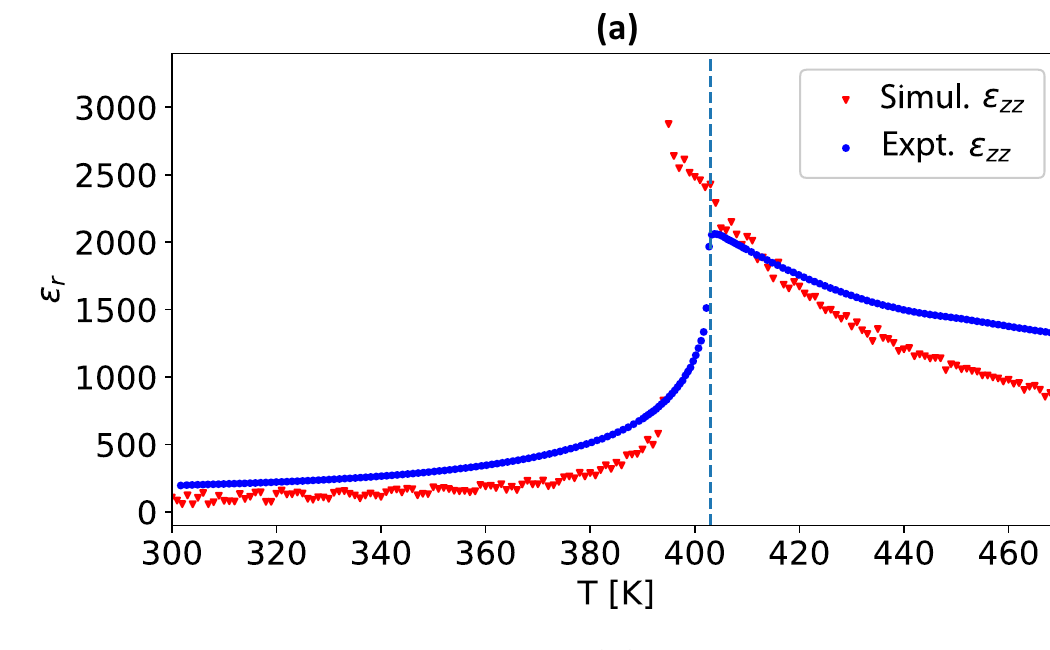
\includegraphics[width=0.46\textwidth]{../soutenance_stage_beamer/assets/mayer2022_fig3a_permittivity.png}
\caption{Permittivité calculée par dynamique moléculaire classique avec le
potentiel effectif enrichi de Mayer \emph{et al.} Cette référence montre que
l'enrichissement par les modes optiques secondaires rapproche fortement la
tendance calculée de la réponse expérimentale ; elle ne constitue pas une
mesure directe. Adapté de la figure~3(a) de la réf.~\cite{Mayer2022}.}
\label{fig:core_mayer_md}
\end{figure}

\begin{figure}[H]
\centering

\includegraphics[width=0.88\textwidth]{mayer_chi_temperature_300_800K_final.png}
\caption{Comparaison de la susceptibilité du mode mou pour les paramètres de
Mayer. Les points sont des mesures numérisées ; les courbes continues ou
pointillées sont des calculs ou des reconstructions empiriques. Les segments
hors intervalle expérimental sont des extrapolations. Données et potentiel :
Mayer et al.~\cite{Mayer2022}.}
\label{fig:ann_mayer_complet}
\end{figure}

Le même critère $A_1\to0^+$ permet de comparer directement les différents
protocoles de pression et les deux jeux de paramètres. Les racines du tableau
suivant sont obtenues par résolution du résidu scalaire, sans extrapolation
linéaire de valeurs calculées de $A_1(T)$.
\begin{table}[H]
\centering
\small
\caption{Limites de stabilité paraélectrique centrée sur la grille de
Brillouin $40^3$. $T_C^{(A_1)}$ désigne la spinodale définie par
$A_1(T)\to0^+$, et non la température de coexistence du premier ordre. Les
lignes Mayer utilisent les paramètres PBEsol après réduction anharmonique.}
\label{tab:core_a1_transition_temperatures}
\renewcommand{\arraystretch}{1.12}
\begin{tabular}{p{0.24\textwidth}p{0.34\textwidth}r r}
\hline
Jeu de paramètres & Protocole de pression &
$T_C^{(A_1)}$ (K) & $p_{\rm eff}(T_C)$ (GPa) \\
\hline
Nishimatsu WC--GGA & $p_{\rm eff}=0$ & $174.7080$ & $0$ \\
& Ajustement ponctuel à $a(T)$ & $198.0939$ & $-0.69308$ \\
& Pression de maille affine $p_a(T)$ & $198.8648$ & $-0.71573$ \\
& Ajustement affine à la réponse $p_\chi(T)$ & $385.1604$ & $-5.74955$ \\
\hline
Mayer PBEsol & $p_{\rm eff}=0$ & $170.6798$ & $0$ \\
& Ajustement ponctuel à $a(T)$ & $172.7661$ & $-0.08324$ \\
& Pression de maille affine $p_a(T)$ & $169.6995$ & $+0.03866$ \\
\hline
\end{tabular}
\end{table}

Deux constats se dégagent. D'une part, l'amélioration obtenue
en dynamique moléculaire confirme que les couplages aux modes optiques
secondaires doivent être considérés dans le diagnostic de l'écart. D'autre
part, la comparaison directe aux résultats expérimentaux montre que la réponse
obtenue avec la fermeture SCHA centrée reste nettement trop rigide. Le meilleur
accord obtenu par la dynamique moléculaire classique de Mayer avec ces mêmes
mesures, pour le même potentiel enrichi, suggère qu'une partie de l'écart peut
provenir de la fermeture statistique, sans l'établir causalement. Ce constat
motive le diagnostic post-SCHA de la section suivante.

Les résultats autorisent à ce stade de l'analyse trois conclusions :
\begin{enumerate}
  \item la correction du seul volume ne rétablit pas la réponse mesurée ;
  \item une correction scalaire de masse reproduit les données sur un intervalle
  restreint, mais cette calibration inverse n'identifie pas le mécanisme absent ;
  \item les modes optiques et leurs couplages anharmoniques sont pertinents en
  dynamique moléculaire ; l'écart restant entre notre SCHA et les mesures est
  compatible avec une limite de la fermeture statistique, sans l'isoler comme
  cause.
\end{enumerate}

% =============================================================================
% =============================================================================
\section{Diagnostic post-SCHA et limites d'interprétation}
\label{ann:post_scha_fr}
% =============================================================================

La motivation de ce calcul vient directement de la comparaison précédente.
La pression imposant le bon paramètre de maille ne rétablit pas la réponse de
BaTiO$_3$, et le potentiel enrichi de Mayer donne en dynamique moléculaire une
transition cubique--tétragonale à $395\,\mathrm K$, proche des
$403\,\mathrm K$ expérimentaux~\cite{Mayer2022}, alors que sa résolution par la
SCHA scalaire centrée reste trop dure. Le volume n'est donc pas le seul
candidat. Comme la SCHA ne conserve que les contractions gaussiennes, le test
naturel suivant consiste à réintroduire la première corrélation irréductible
qu'elle ne resomme pas, puis à vérifier sa taille. Cette correction sert
uniquement à tester le signe et l'ordre de grandeur de l'effet ; elle n'est pas
utilisée à des fins prédictives.

Pour organiser cette question, on réécrit exactement le Hamiltonien sous la
forme
\begin{equation}
H=H_{\rm SCHA}
+\epsilon\left[
V(\mathbf P)+\frac12\,\mathbf P\mathbin{\cdot}(A_0-A_{\rm SCHA})
\mathbin{\cdot}\mathbf P
\right].
\label{eq:core_post_scha_reorganization}
\end{equation}
Ici $H_{\rm SCHA}=H_{\rm cin}+\tfrac12\mathbf P\cdot A_{\rm SCHA}\cdot\mathbf P$
est le Hamiltonien de référence gaussien, et $A_0$ le noyau quadratique
microscopique nu, exprimé dans la même convention de polarisation que
$A_{\rm SCHA}$. $V(\mathbf P)$ désigne la partie anharmonique du Hamiltonien
exact ; $\epsilon$ est un paramètre formel de comptage fixé à $1$ à la fin.
L'identité redonne alors exactement
$H=H_{\rm cin}+\tfrac12\mathbf P\cdot A_0\cdot\mathbf P+V$.
Le crochet est l'interaction résiduelle
$\Delta V_{\rm SCHA}=V+\tfrac12\mathbf P\cdot(A_0-A_{\rm SCHA})\cdot\mathbf P$.
Comme le noyau SCHA satisfait les équations de stationnarité dans la famille
gaussienne retenue, il est raisonnable d'espérer que ce reste soit
plus petit que l'interaction anharmonique initiale et qu'une expansion en
$\epsilon$ soit informative. Cette espérance doit être vérifiée a posteriori par la taille des corrections, notamment le rapport $r$ introduit ci-dessous.

Après soustraction des insertions déjà absorbées dans la SCHA, la correction
irréductible la moins coûteuse du propagateur contient deux vertex quartiques
et trois lignes internes. Sous forme condensée,
\begin{equation}
\begin{aligned}
[\Sigma_{44}^{(2)}(K)]_{ab}
=-\frac{1}{6}\int_{Q_1,Q_2}
[\overline\Gamma_4]_{acde}\,
G^{cf}_{\mathrm{SCHA}}(Q_1)
G^{dg}_{\mathrm{SCHA}}(Q_2)\\
\times G^{eh}_{\mathrm{SCHA}}(-K-Q_1-Q_2)
[\overline\Gamma_4]_{bfgh}.
\end{aligned}
\label{eq:ann_sunset}
\end{equation}

Le vertex $\overline\Gamma_4$ utilisé ici est la dérivée quatrième locale
moyennée dans la mesure gaussienne : il comprend le quartique projeté après
élimination de la déformation homogène et les contractions locales des termes
sextiques et octiques. Les vertex dynamiques issus de la déformation
inhomogène, les autres squelettes à deux insertions et le résidu quadratique
non local de la fermeture restreinte sont omis. Le calcul ne constitue donc
pas le développement post-SCHA complet à cet ordre. La petite quantité pertinente n'est pas l'écart visuel
entre deux courbes, mais\footnote{La notation $\lVert\cdot\rVert_2$ utilisée
dans l'équation suivante désigne la norme spectrale, c'est-à-dire la plus grande
valeur singulière. Pour la matrice symétrique considérée ici, elle est égale au
plus grand module de ses valeurs propres.}
\begin{equation}
r(K)=\left\|
A_{\rm SCHA}(K)^{-1/2}
\Sigma_{44}^{(2)}(K)
A_{\rm SCHA}(K)^{-1/2}
\right\|_2 .
\label{eq:core_post_scha_control_ratio}
\end{equation}
Une insertion unique n'est interprétable comme correction perturbative que si
$r\ll1$ sur la région de moment et de température qui contrôle l'observable.
Lorsque $r\gtrsim1$, son signe indique encore le type de corrélation manquante,
mais sa valeur ne peut être ajoutée quantitativement au propagateur.

L'évaluation déplace la réponse vers l'expérience, mais la norme de
la correction rapportée au noyau de départ dépasse l'unité dans l'intervalle
étudié. Elle constitue donc un diagnostic de corrélations non gaussiennes
manquantes, et non une prédiction exploitable en tant que telle. Une resommation cohérente ou le
calcul de la courbure de l'énergie libre optimisée doit précéder toute
interprétation quantitative.

Sur les points de Mayer numérisés entre 400 et $470\,\mathrm K$, cette
correction linéarisée réduit le désaccord d'environ $48\,\%$ à pression nulle et de
$65\,\%$ sur le fond à maille ajustée. Le mouvement est donc nettement dans le
bon sens, mais le rapport $r$ reste supérieur à l'unité : l'amélioration
visuelle diagnostique une physique non gaussienne manquante sans établir la
convergence de l'expansion.

\begin{figure}[H]
\centering

\includegraphics[width=0.92\textwidth]{mayer_post_scha_quartic_one_shot_400_800K_n40.png}
\caption{Diagnostic quartique local projeté en une passe autour de la solution
SCHA paramétrée par Mayer. La correction rapproche la réponse de l'expérience,
mais le rapport de contrôle dépasse l'unité : aucune prédiction de type Dyson
n'est revendiquée. Comparaison fondée sur Mayer et al.~\cite{Mayer2022}.}
\label{fig:cs_post_scha}
\end{figure}

L'ordre de travail retenu est donc : (i) calculer la courbure exacte de
$F_{\rm SCHA}[\overline P]$ après réoptimisation du noyau ; (ii) construire les
vertex cohérents associés à cette énergie libre ; (iii) tester une resommation
2PI ou de Dyson ; (iv) n'introduire un groupe de renormalisation du mode de
Matsubara nul que si l'action de départ et le raccord ultraviolet sont
contrôlés.

% =============================================================================
\section{Approximation de cristal virtuel pour le BST}
\label{ann:bst_vca_fr}
% =============================================================================

L'isovalence de Ba et Sr motive une première interpolation homogène, sans
justifier à elle seule la linéarité de tous les paramètres. La VCA ne décrit
toutefois ni les fluctuations locales de composition ni le désordre qu'elles
induisent.
\begin{figure}[H]
\centering

\includegraphics[width=0.70\textwidth]{periodic_table_ba_sr.png}
\caption{Repérage chimique de Sr et Ba : les deux éléments appartiennent au
groupe 2 des alcalino-terreux. Cette parenté motive l'interpolation VCA, sans
annuler les différences de masse, de rayon ionique ou d'environnement local.}
\label{fig:core_vca_periodic_table}
\end{figure}

Pour une composition $x$ en baryum, la VCA interpole les paramètres
microscopiques indépendants,
\begin{equation}
\lambda(x)=x\lambda_{\mathrm{BTO}}+(1-x)\lambda_{\mathrm{STO}},
\label{eq:ann_vca_interp}
\end{equation}
puis reconstruit les quantités dépendantes telles que les inverses élastiques et
les facteurs de conversion. Cette procédure conserve l'invariance par
translation et permet de réutiliser le solveur $3\times3$ pour chaque $k$.

L'interpolation porte uniquement sur les données microscopiques indépendantes :
$a_0$, $M^*$, $Z^*$, $\varepsilon_\infty$, $K_2$, $j_1,\ldots,j_7$, les six
coefficients élastiques et de couplage indépendants, puis les invariants locaux
d'ordres quatre, six et huit. À chaque composition, le code recalcule ensuite
\begin{equation}
\Omega_0(x)=a_0(x)^3,\qquad
s(x)=\frac{\Omega_0(x)}{Z^*(x)},\qquad
\Lambda^{\rm hom}(x)=B(x)^T\mathcal B(x)^{-1}B(x),
\label{eq:core_vca_reconstructed_quantities}
\end{equation}
ainsi que le facteur dipolaire
$Z^*(x)^2/[\varepsilon_\infty(x)\Omega_0(x)]$, le noyau d'Ewald et tous les
coefficients exprimés en polarisation. Interpoler directement
$\Lambda^{\rm hom}$, $B^{-1}$ ou les cinq $A_{0,i}$ donnerait en général un
résultat différent et incohérent avec les entrées.

La cellule virtuelle étant identique en tout site, la covariance conserve la
forme
\begin{equation}
G_x^{ab}(T)=\frac{\Omega_0(x)}{(2\pi)^3}
\int_{\rm BZ(x)}\mathrm d^3k
\frac{1}{\beta}\sum_n[A_x(\mathbf k,\omega_n;T)^{-1}]^{ab}.
\label{eq:core_vca_propagator}
\end{equation}
Toute introduction d'un désordre chimique explicite aurait
pour conséquence que le solveur $3\times3$ n'est plus suffisant.

Pour les fractions
de baryum $x=0.4$, $0.5$ et $0.6$, une correction affine ajustée entre 400 et
$600\,\mathrm K$ reconstruit la cible nominale de Curie--Weiss avec un résidu
maximal inférieur à $0.62\,\%$. Ce résidu quantifie seulement l'ajustement affine
à deux paramètres ; il ne valide pas le mécanisme physique. Les cibles nominales
sont des reconstructions contraintes par la littérature, et non des mesures
brutes directes.

\begin{figure}[H]
\centering

\includegraphics[width=0.96\textwidth]{chi_temperature_bst_vca_x040_060_300_600K_n40.png}
\caption{Réponse VCA--SCHA invariante par translation pour trois compositions
de BST. Les courbes nominales de Curie--Weiss sont des reconstructions
contraintes par la littérature, non des mesures brutes directes, et les
corrections affines sont des calibrations inverses. Contexte expérimental :
Weerasinghe et al.~\cite{Weerasinghe2013}.}
\label{fig:cs_bst_response}
\end{figure}

Sur les trois compositions représentées, la prédiction à $p_{\rm eff}=0$
semble s'améliorer lorsque la fraction de Sr augmente, c'est-à-dire lorsque la
fraction de Ba décroît de $x=0.6$ à $x=0.4$. Cette observation doit rester
prudente : elle peut relever de la plage limitée de compositions considérée ou
de la reconstruction empirique utilisée comme cible. Une interprétation
physique plausible est néanmoins que l'ajout de Sr abaisse la température de
transition ; à température donnée, le système est alors plus éloigné de la
région de ramollissement et les effets anharmoniques et non gaussiens les plus
marqués peuvent peser moins fortement sur la réponse. Cette lecture est
compatible avec l'efficacité des phonons auto-cohérents documentée pour la
phase cubique de SrTiO$_3$, rappelée en
\hyperref[ann:scha_reponse]{\textcolor{blue}{section~\ref*{ann:scha_reponse}}}~\cite{TadanoTsuneyuki2015}. Elle ne démontre
toutefois ni que l'amélioration soit monotone en composition, ni que
l'éloignement de la transition en soit l'unique cause.
